\section{Conceptos}


\subsection{¿Qué es Git?}

Es un software de control de versiones creado por el desarrollador de Linux: Linus Torvalds, es un software libre.

Funciona para tener un control, dar mantenimiento y desarrollar aplicaciones de forma individual, como en equipo.

Logra estas características de  desarrollo, mantenimiento y control guardando, en un registro, todos los cambios que sufre un archivo o conjunto de archivos.


\subsection{Funcionamiento de Git}

Supongamos que tenemos un archivo \textit{index.html}, al principio tiene 0 líneas de código, después de dos horas, ya tiene más de 100 líneas y decidimos guardamos el progreso, entonces, al principio del trabajo, nuestro archivo era una versión (sin nada), después de las dos horas, ya es otra versión completamente distinta, Git se encarga de registrar las versiones que se van creando cuando uno decide que ha concluido con una versión, con una jornada laboral, o con un requisito de una lista de trabajo, estos registros tiene forma de “instantánea” (como una foto), la cual está compuesta por un código alfanumérico, por ejemplo: 8745dsd; y un mensaje entre comillas ("") que la describe, como lo podría ser: "Comienzo del proyecto".

Conforme vayamos trabajando el archivo y guardando los cambios, se irán creando más instantáneas de nuestro trabajo, como vemos en la \textit{Figura \ref{fig: 1}}:
\begin{figure}[H]
    \centering
    \caption{Ilustración de versiones de un archivo}
    \label{fig: 1}
    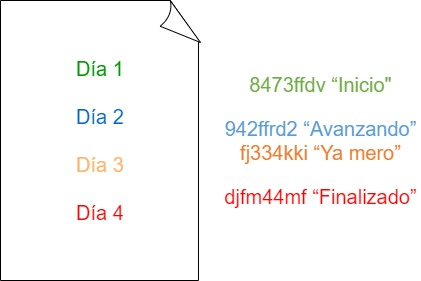
\includegraphics[width=8cm]{conceptos/g1.jpg}
\end{figure}

Git guarda las instantáneas que tiene de nuestro trabajo, así que, si durante el día 10 de trabajo, algo falla, podemos regresar a la instantánea de nuestro archivo en el día 7, para revisar que salió mal. Esto es muy útil para proyectos con muchos archivos.


\subsection{Estructura de un repositorio local}

Cuando decidimos crear un directorio local con un proyecto personal o grupal, al utilizar el comando \textbf{git init}, en nuestro directorio, se crea una carpeta invisible llamada\textbf{ .git}, la cual está constituida por dos partes: el \textbf{área de ensayo} y el \textbf{repositorio local}, el primero nos muestra todos aquellos archivos o ficheros que tienen seguimiento, es un área temporal; la segunda área almacena todos los archivos que tienen seguimiento y que están listos para que se les tome una \textit{instantánea}. La \textit{Figura \ref{fig: 2}} puede dar a entender un poco más este concepto:
\begin{figure}[H]
    \centering
    \caption{Paso entre la estructura de un repositorio local}
    \label{fig: 2}
    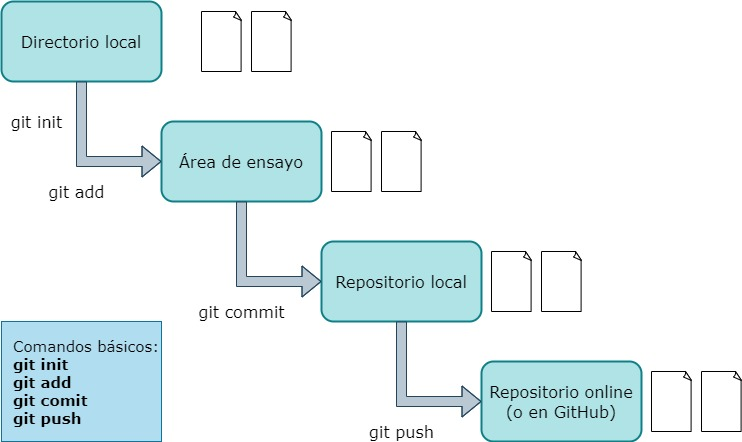
\includegraphics[width=\textwidth]{conceptos/g2.jpg}
\end{figure}

\textit{Nota}:los comandos básicos serán explicados más adelante.


\subsection{Ramas}

Una \textbf{rama} es una copia de un archivo (que viene de un original) o archivos de nuestro repositorio local que es trabajada por un usuario o usuarios en específico, Git te permite crear más de una \textit{rama} para que más de una persona o grupos trabaje en un archivo o archivos del proyecto, así, abarcando más tareas y trabajando más rápido, al final, cuando los usuarios terminaron su trabajo, Git puede unificar y combinar todas las ramas para que sea un solo archivo, archivos o repositorio con todo el trabajo de todos los usuarios.

En caso de que, varios usuarios hayan modificado en sus ramas el mismo archivo en la misma sección de código, a la hora de unificar todas las ramas, habrá un conflicto donde Git avisa y pregunta qué se hará en ese caso. Una rama podría tener el siguiente aspecto de la \textit{Figura \ref{fig: 3}}, para que sean más fáciles de visualizar y entender:
\begin{figure}[H]
    \centering
    \caption{Ejemplificación de dos ramas de un repositorio}
    \label{fig: 3}
    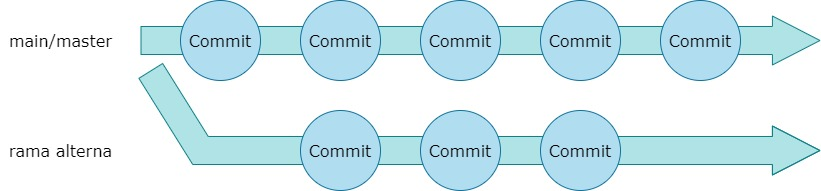
\includegraphics[width=\textwidth]{conceptos/g3.jpg}
\end{figure}

Vemos que la rama \textit{main/master} es la principal o la origen, a partir del primer \textbf{commit}, nace una \textbf{rama alterna} que es exactamente igual a la rama main/master, sin embargo, lo que se haga en esta última no afecta a su rama alterna, del mismo modo que lo que se haga en la rama alterna no afecta a su rama origen o principal.

Las ramas más comunes son \textbf{main} y \textbf{master}.

Trabajando en consola y sin utilizar un editor de texto, para poder crear una rama nueva en nuestro repositorio local, utilizamos el comando \textbf{git branch [nombre]}; puede usar el comando \textbf{git status -s} para ver el registro de la creación de la rama y \textbf{git branch} para ver las ramas existentes en el repositorio; puede utilizar el comando \textbf{git checkout [nombre rama]} para moverse a una rama existente para poder trabajar sobre ella.

\textbf{Observación:} en caso de que se esté trabajando en una rama ajena a main o master (por ejemplo, \textit{rama v2.1}) y se desee volver a main, usando el comando \textbf{git checkout [nombre rama]}, en algunos editores de texto, como Dreamweaver, se nos notificará que se han hecho cambios desde fuera del editor de texto, por lo que podemos cargarlos en nuestro proyecto, sabemos que en main no hemos realizado cambios, pero si en v2.1, entonces, al pasa a una rama sin dichos cambios, se nos notifica en algunos editores de texto. Esto es una consideración a tomar en cuenta al moverse entre ramas.

Para poder mezclar, combinar o unir el trabajo de varias ramas en una sola, es requerido primero estar en la rama principal (main o master), se utiliza el comando \textbf{git merge [nombre rama]}, en caso de que se hayan modificado el mismo archivo en líneas de código similares o iguales, lanzará un error diciendo donde está ubicado el error, para que nosotros determinemos que solución dar.


\subsection{Tags}

Las \textbf{tags} (etiquetas) son identificadores que determinan hasta un cierto punto nuestro repositorio online, es decir, si tenemos 20 archivos que conforman nuestro repositorio, a estos 20 archivos los podemos denominar como “versión 1.0”, entonces, utilizamos estas etiquetas para definir la versión del repositorio y poder hacer que la gente vea en qué versión se encuentra nuestro trabajo, y poder descargarla. Estas etiquetas funcionan también para indicar que nuestro repositorio está \textit{en proceso} o \textit{terminado}.

Para poder crear una etiqueta en consola escribimos el comando \textbf{git tag [nombre] “descripción”} (por ejemplo: \textit{git tag 5-5-20v1 “versión 1.0”}), en este momento, solo hemos creado la etiqueta, podemos apreciarlo usando el comando \textbf{git status -s}, todavía falta subirla, para ello, usando el comando \textbf{git push tags}.



\section{Comandos de Git}

Enlistamos todos los comandos vistos en el curso de YouTube que aprendimos.
\begin{itemize}
    \item Comandos para comenzar a trabajar con un repositorio local:
    \begin{itemize}
        \item \textbf{git init:} comienza el seguimiento de versiones del proyecto o archivos, en el directorio donde está nuestro trabajo.
        \item \textbf{git add \textit{[archivo]}:} es usado para darle seguimiento a un o unos archivos, los archivos que sean agregados pasan al área de ensayo. P. e: \textit{git add index.php}.
        \item \textbf{git add .: }les da seguimiento a todos los archivos de una carpeta.
        \item \textbf{git commit -m “\textit{mensaje}”:} pasa todos los archivos del área de ensayo al repositorio local, una vez estando ahí, toma la instantánea de los archivos. P. e: \textit{git commit -m “Primer avance”}.
        \item \textbf{git commit -am “\textit{mensaje}”:} agrega todos los archivos que han sido modificados recientemente del área de ensayo al repositorio local, una vez estando ahí, toma la instantánea de los archivos.
        \item \textbf{git status -s: }enlista todos los archivos que tienen seguimiento o si están en el área de ensayo.
        \item \textbf{git log –oneline: }enlista todas las instantáneas creadas de nuestro proyecto.
        \item \textbf{git reset –hard \textit{[código instantánea]}:} regresa a una instantánea creada previamente. P. e: \textit{git reset –hard 90ffrtyu}.
        \item \textbf{git remote add origin \textit{[dirección repositorio online]}.git:} a esta dirección se va a subir nuestro repositorio local. Debe haber primero ingresar las credenciales de su cuenta donde está el repositorio utilizando los siguientes comandos:
        \begin{itemize}
            \item \textbf{git config –global user.name “\textit{nombre usuario GitHub}”}
            \item \textbf{git config –global user.email “\textit{correo electrónico GitHub}”}
        \end{itemize}
    \end{itemize}
    \item Comandos para ramas:
    \begin{itemize}
        \item \textbf{git branch:} enlista todas las ramas creadas o existentes hasta el momento.
        \item \textbf{git branch \textit{[nombre]}:} crea una nueva rama en el repositorio local.
        \item \textbf{git checkout \textit{[nombre rama]}:} pasamos a trabajar a la rama seleccionada.
        \item \textbf{git brand -d \textit{[nombre rama]}:} elimina la rama seleccionada.
        \item \textbf{git merge \textit{[nombre rama]}:} comienza el proceso de unificar varias ramas en una sola. En caso de que se hayan hecho cambios en un mismo archivo desde varias ramas (problema de concurrencia), Git lanzará mensaje de error y no podrá concretar la mezcla hasta que nosotros lo resolvamos.
        \item \textbf{git branch -M main: }asigna a qué rama se va a subir el repositorio local.
        \item \textbf{git push -u origin main:} sube todo el contenido del repositorio local al de la dirección web.
    \end{itemize}
    \item Comandos para subir y clonar repositorios:
    \begin{itemize}
        \item \textbf{git pull: }jala todo el contenido de un repositorio online a nuestro repositorio local. En caso de que muestre algún error al escribir este comando, al final del mismo, agregue la dirección .git del repositorio online.
        \item \textbf{git clone \textit{[dirección .git]}:} clona o copia los archivos de un repositorio online a un directorio local de nuestra computadora.
        \item \textbf{git push tags: }sube todas las etiquetas creadas del repositorio local al online.
    \end{itemize}
\end{itemize}



\section{Trabajando con Git en consola}

Los siguientes puntos describen el proceso de trabajo con Git utilizando solamente el software oficial de Git en nuestro sistema operativo, usando además un editor de texto como auxiliar, más adelante se describirá el uso de Git con un editor de texto mejorado y botones que facilitan el uso y comprensión de Git.
\begin{enumerate}
    \item Creamos un directorio local en nuestro sistema operativo para nuestro proyecto.
    \item Debemos instalar Git en nuestra máquina (\underline{https://git-scm.com/downloads}).
    \item Una vez instalado, debemos tener a la mano un editor de texto para poder crear los archivos de nuestro proyecto en nuestro directorio local (Notepad++, Bloc de Notas, Visual Studio Code, Dreamweaver, etc.).
    \item Creamos un archivo en nuestro directorio local, ya sea por medio del Explorador de archivo de nuestro sistema operativo o por el editor de texto, crearemos un archivo llamado \textit{index.html}.
    \item Abriremos la consola Git Bash en la ubicación donde está nuestro directorio local (en Windows, clic derecho sobre cualquier parte vacía del directorio, y damos clic en la opción \textbf{Git Bash Here}), con esto podremos trabajar Git en el directorio local.
    \item Para no entrar en detalle sobre cuántos y qué es lo que contienen los archivos de este proyecto ejemplo, el archivo \textit{index.html} tiene como contenido la estructura básica de un archivo html, este será la primera versión o instancia de nuestro proyecto en Git.
    \item En la consola Git Bash, escribimos el comando \textbf{git init}, recordemos que la consola está ubicada en el directorio local de nuestro proyecto, por lo que, Git creará una carpeta escondida \textbf{.git}, donde estará la información necesaria para crear el repositorio local.
    \item Si escribimos el comando \textbf{git status -s} veremos la lista de los archivos en el directorio local de nuestro proyecto, pero como ninguno ha sido agregado al área de ensayo ni tienen seguimiento, para lograr esto, debemos escribir el comando \textbf{git add index.html}, repetimos el comando \textbf{git status -s} y ahora si nuestro único archivo tiene seguimiento.
    \item Escribimos el comando \textbf{git commit -m “Primer avance”} para crear la primer instantánea o versión de nuestro proyecto, este comando manda nuestro archivo \textit{index.html} al repositorio de Git. Si escribimos el comando \textbf{git log –oneline} veremos la instantánea que acabamos de crear, con su código y mensaje.
    \item Si volvemos a escribir el comando \textbf{git status -s}, veremos que \textit{index.html} ya no está presente, esto es debido a que ahora está ubicado en el repositorio, no en el área de ensayo.
    \item Ahora bien, si realizamos cualquier cambio en \textit{index.html} (por ejemplo, agregar un Header 1 con un mensaje de bienvenida), y escribimos el comando \textbf{git status -s}, veremos que este volverá a ser listado como un archivo en el directorio local, pero debe estar en el área de ensayo para que podamos realizar un commit nuevamente, repetimos el comando \textbf{git add index.html} para que este tenga seguimiento nuevamente.
    \item Repetimos el comando \textbf{git commit -m “Segundo avance”} para crear otra instantánea con nuestras modificaciones.
    \item En github.com, debemos tener un repositorio de prueba creado y su enlace a la mano, para poder subir desde la consola todos los archivos del repositorio local al que está ubicado en GitHub. Primero debemos configurar a qué cuenta y repositorio se va a subir el repositorio local, para ello, escribimos los comandos \textbf{git config –global user.name} y \textbf{git config –global user.email}, después de las últimas palabras de cada comando, debemos escribir el nombre de usuario y correo electrónico de la cuenta de GitHub a donde se subirá el proyecto, después de configurarlos, escribimos el comando \textbf{git remote add origin}, al final de este comando, va la dirección \textbf{.git} de nuestro repositorio (se encuentra en la página principal del repositorio online de GitHub), después escribimos el comando \textbf{git branch -M main}, este comando indica a qué rama se subirá el repositorio local, preferiblemente lo haremos a la rama \textbf{main}, ya que si no se establece este comando, se subirá en automático a la rama \textbf{master}, finalmente, escribimos el comando \textbf{git push -u origin main}, este comando se encarga de subir el repositorio local a GitHub. Una vez hayamos hecho todo esto, podemos refrescar nuestro repositorio en GitHub para ver nuestro proyecto en línea.
    \item En caso de que se haga alguna modificación desde GitHub en el repositorio online, podemos obtener los archivos o modificaciones online en nuestro repositorio local, para ello, utilizamos el comando \textbf{git pull} o \textbf{git pull \textit{[dirección .git]}}, para obtener los archivos modificados, siempre y cuando en la consola ya estemos trabajando en el directorio local.
    \item En caso de que hayamos perdido nuestro proyecto de directorio local, podemos utilizar el comando \textbf{git clone} para poder copiar todo lo que esté en un directorio online a nuestra computadora, y así seguir trabajando en la última versión que realizamos. Refrescamos la pestaña de GitHub en nuestro navegador, y veremos que ya existe una versión 1.0 de nuestro proyecto.
\end{enumerate}



\section{Trabajando con Git en Visual Studio Code y consola}

Visual Studio Code (VSC a partir de ahora) cuenta, de manera nativa, con herramientas Git para poder crear repositorios locales y poderlos subir a GitHub de una manera muy visual y fácil de comprender.

Primero que nada, debemos tener nuestro directorio local con nuestro proyecto en el sistema operativo, en VSC, es recomendable crear \textbf{áreas de trabajo} o \textbf{Workspaces} para nuestro directorio local, en caso de que se cierre accidentalmente VSC, cargamos nuestro área de trabajo y todo estará justo como lo dejamos.

Las siguientes Figuras muestran como crear un \textit{Workspace}:
\begin{figure}[H]
    \centering
    \caption{Agregando directorio local a VSC}
    \label{fig: 4}
    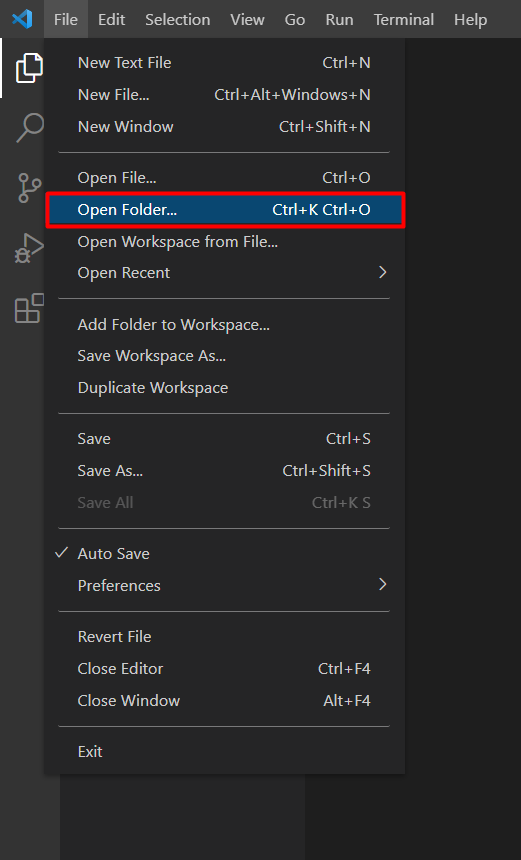
\includegraphics[height=12cm]{capturas/creando_w1.png}
\end{figure}
\begin{figure}[H]
    \centering
    \caption{Seleccionando directorio local}
    \label{fig: 5}
    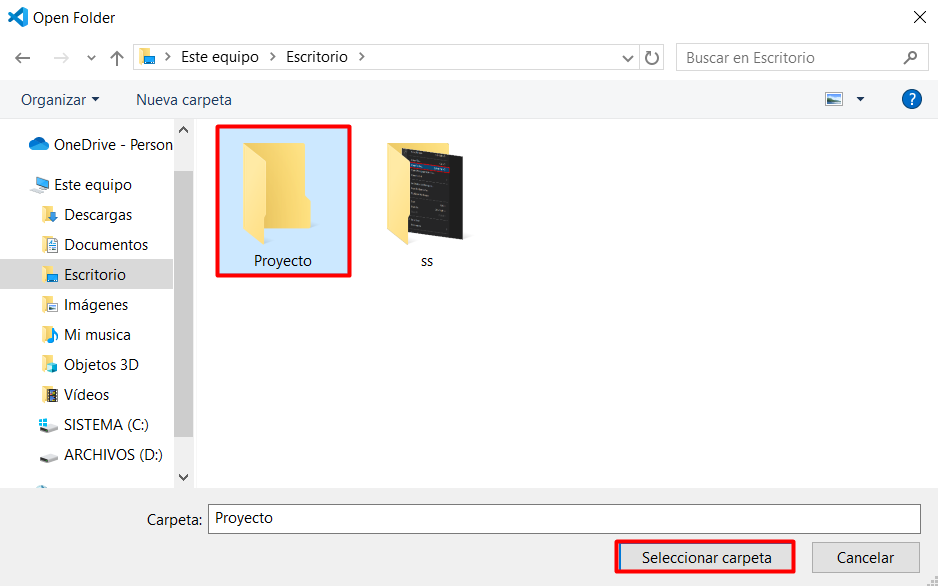
\includegraphics[width=12cm]{capturas/creando_w2.png}
\end{figure}
\begin{figure}[H]
    \centering
    \caption{Autorizando directorio local en VSC}
    \label{fig: 6}
    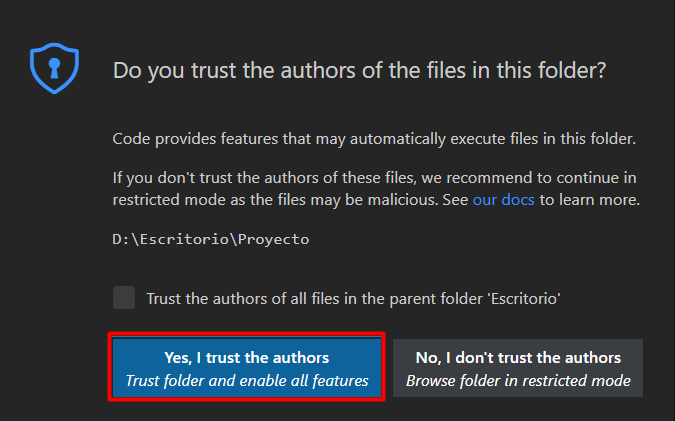
\includegraphics[width=10cm]{capturas/creando_w3.png}
\end{figure}
\begin{figure}[H]
    \centering
    \caption{Agregando Workspace a VSC}
    \label{fig: 7}
    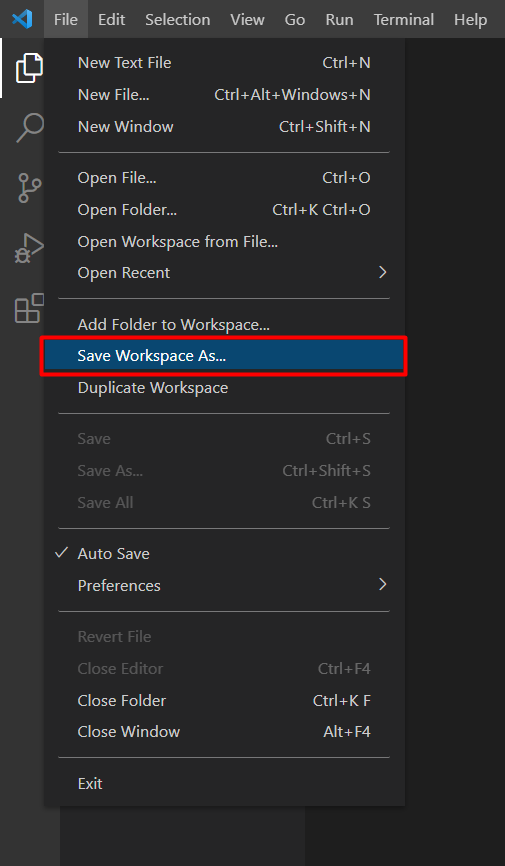
\includegraphics[height=12cm]{capturas/creando_w4.png}
\end{figure}
\begin{figure}[H]
    \centering
    \caption{Seleccionando dirección donde guardar Workspace y nombrándolo}
    \label{fig: 8}
    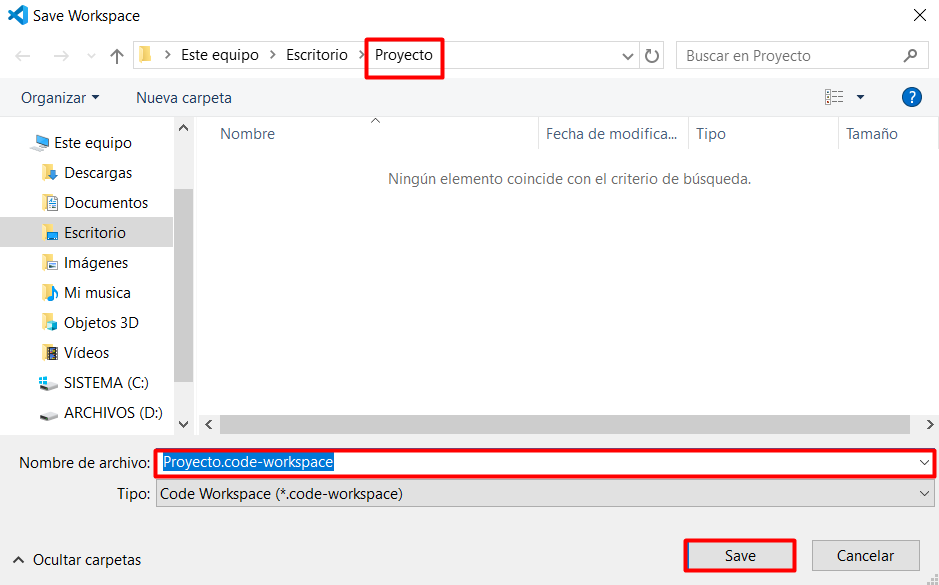
\includegraphics[width=12cm]{capturas/creando_w5.png}
\end{figure}

Vemos que en la \textit{Figura \ref{fig: 4}} y \textit{\ref{fig: 5}} se abre y ubica el directorio local de nuestro proyecto en VSC, la \textit{Figura \ref{fig: 6}} muestra un mensaje (puede aparecer o no) donde confirmamos que confiamos en este directorio, una vez cargado el directorio en VSC, debemos guardarlo como un \textit{área de trabajo}, la \textit{Figura \ref{fig: 7}} lo guarda como tal y la \textit{Figura \ref{fig: 8}} le da una ubicación y nombre al área de trabajo, puede estar ubicado en el mismo directorio local de nuestro proyecto y tener el mismo nombre, o no.

Para \textbf{abrir} un Workspace en VSC se siguen las siguientes Figuras:
\begin{figure}[H]
    \centering
    \caption{Opción para abrir un Workspace}
    \label{fig: 9}
    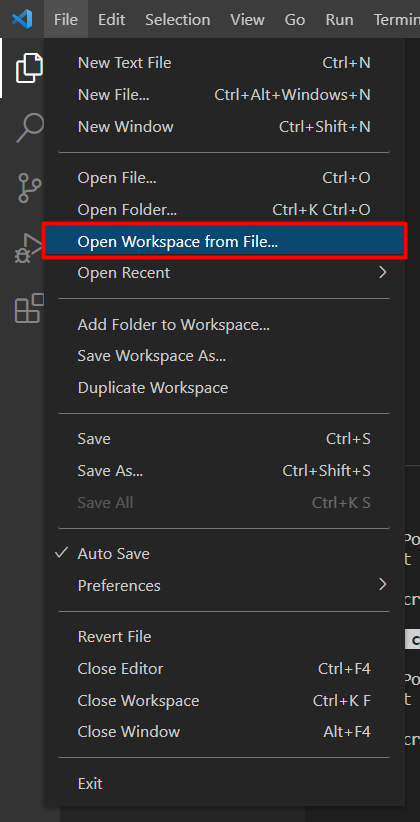
\includegraphics[width=7cm]{capturas/abriendo_w1.png}
\end{figure}
\begin{figure}[H]
    \centering
    \caption{Buscando el Workspace en su ubicación}
    \label{fig: 10}
    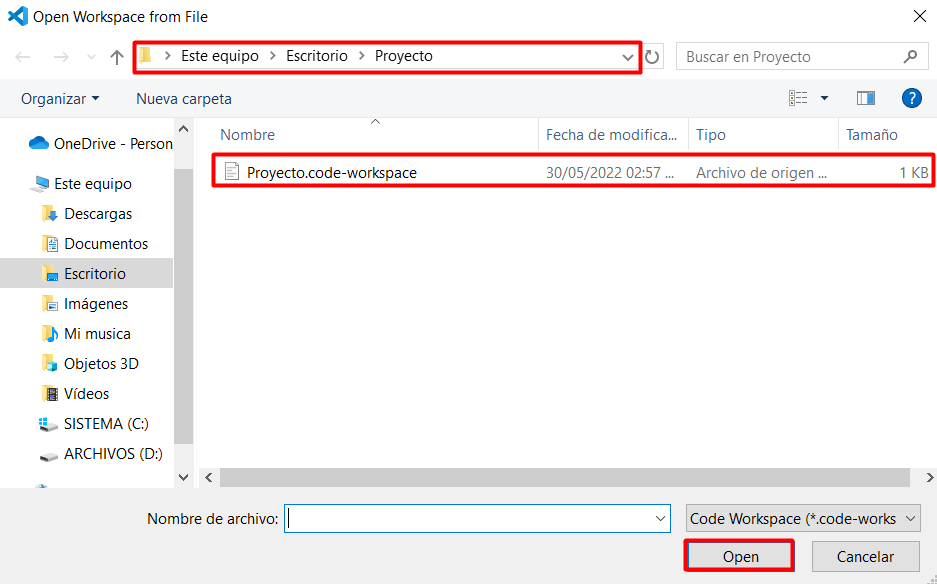
\includegraphics[width=12cm]{capturas/abriendo_w2.png}
\end{figure}

En la misma pestaña \textbf{File} se encuentra la opción para abrir un Workspace desde un archivo, como se ve en la \textit{Figura \ref{fig: 9}}, tendremos que buscar nuestro archivo de .code-workspace donde lo almacenamos, como podemos apreciar en la \textit{Figura \ref{fig: 10}}.

Todo el proceso anterior fue para poder cargar nuestro directorio local a VSC, ahora, es momento de que Git le comience a dar seguimiento. Agregamos al Workspace un archivo \textit{intdex.html}. Si recordamos como fue realizado ese proceso en consola, son prácticamente los mismos comandos, pero VSC te lo muestra de una manera más visual: la \textit{Figura \ref{fig: 11}} muestra que podemos abrir terminales (consolas) en nuestro editor de texto.
\begin{figure}[H]
    \centering
    \caption{Abriendo terminal en VSC}
    \label{fig: 11}
    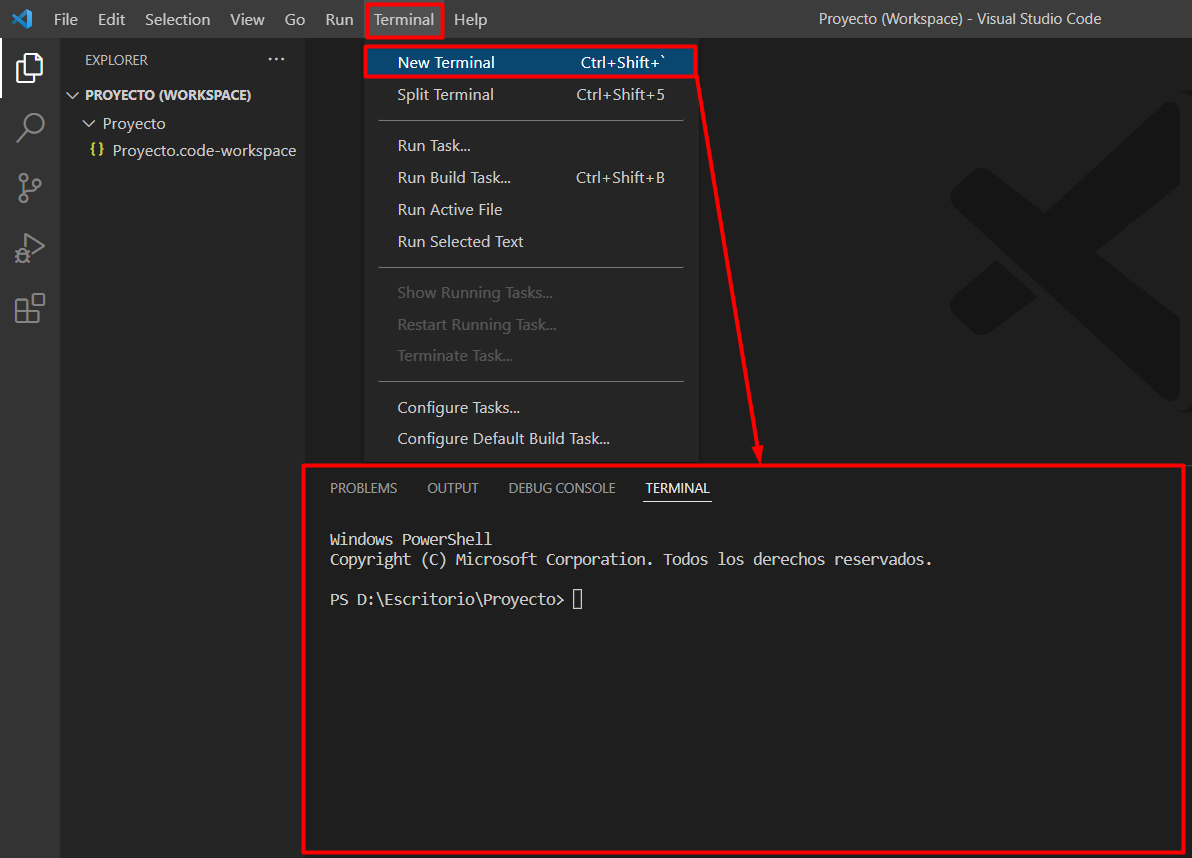
\includegraphics[width=12cm]{capturas/abriendo_terminal.png}
\end{figure}

En esta terminal, escribiremos los comandos git vistos anteriormente, comenzaremos con \textbf{git init}. Vemos en la \textit{Figura \ref{fig: 12}} que el explorador de nuestro Workspace se ha coloreado en verde, y han aparecido algunas letras al lado de los archivos, estas serán explicadas más adelante.
\begin{figure}[H]
    \centering
    \caption{Workspace con Git sin seguimiento}
    \label{fig: 12}
    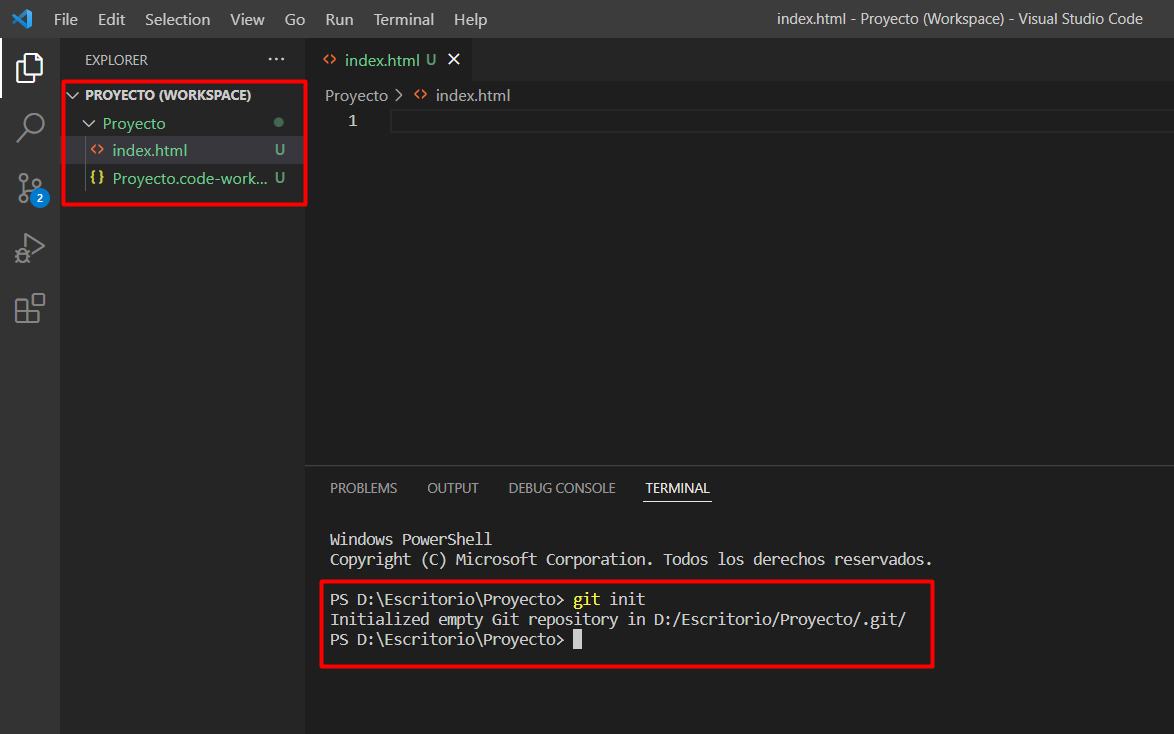
\includegraphics[width=12cm]{capturas/git init.png}
\end{figure}

Entonces, debemos agregar \textit{index.html} al área de ensayo, dándole seguimiento, con el comando \textbf{git add index.html}, una vez hecho esto, podemos realizar un primer commit (aunque el archivo esté vacío) usando el comando \textbf{git commit -m "Primer avance"}, como se ve en la \textit{Figura \ref{fig: 13}}.
\begin{figure}[H]
    \centering
    \caption{Seguimiento y commit de un archivo}
    \label{fig: 13}
    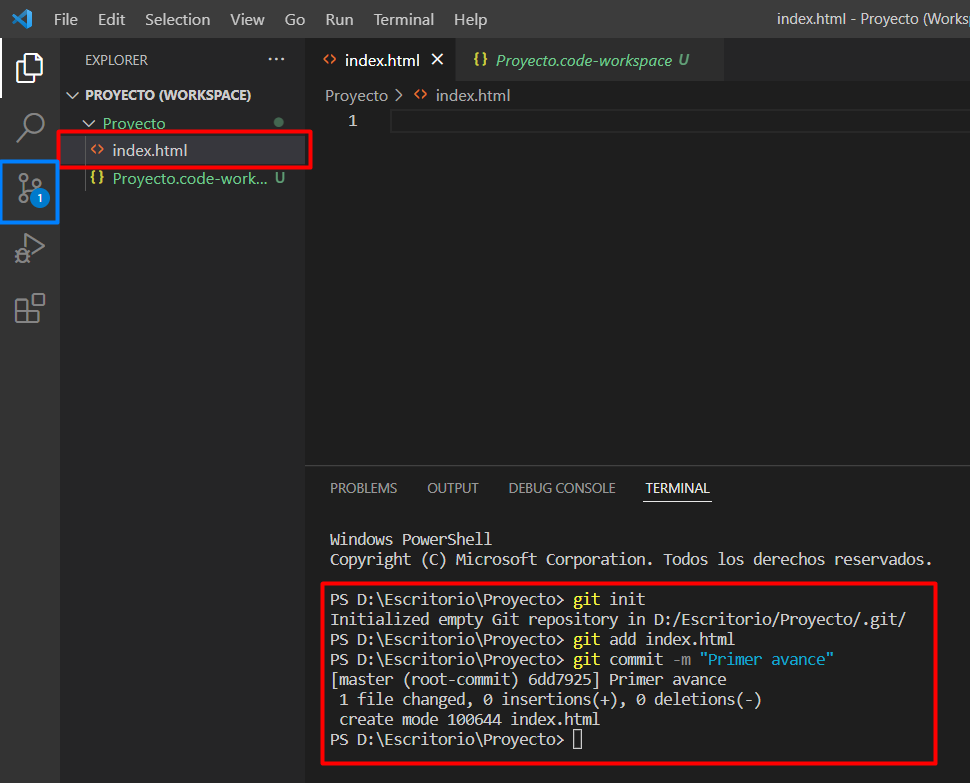
\includegraphics[width=12cm]{capturas/git add git commit.png}
\end{figure}

Si nos fijamos, encerramos una opción en el menú lateral izquierdo con un cuadrado azul, esta opción nos muestra todos aquellos archivos que no tienen seguimiento o que han sido modificados recientemente, por lo que necesitan que se les realice alguna acción o tarea, esta opción es como una lista de archivos a los cuales darles seguimiento en VSC, cuando usamos el comando \textbf{git init}, esta opción tenía 2 tareas o 2 archivos con pendiente para realizar seguimiento: \textit{index.html} y \textit{Proyecto.code-workspace}, al darle seguimiento a index.html nada más, esta lista de tareas bajó a 1, al segundo archivo mencionado no se le hará seguimiento. Vemos entonces, en la \textit{Figura \ref{fig: 14}} que en nuestro explorador de Workspace, el archivo index.html ya no tiene la letra U a su costado, ni está coloreado de verde, esto es porque ya tiene seguimiento, al realizar alguna modificación, este archivo volverá a estar coloreado.
\begin{figure}[H]
    \centering
    \caption{Seguimiento y commit de un archivo}
    \label{fig: 14}
    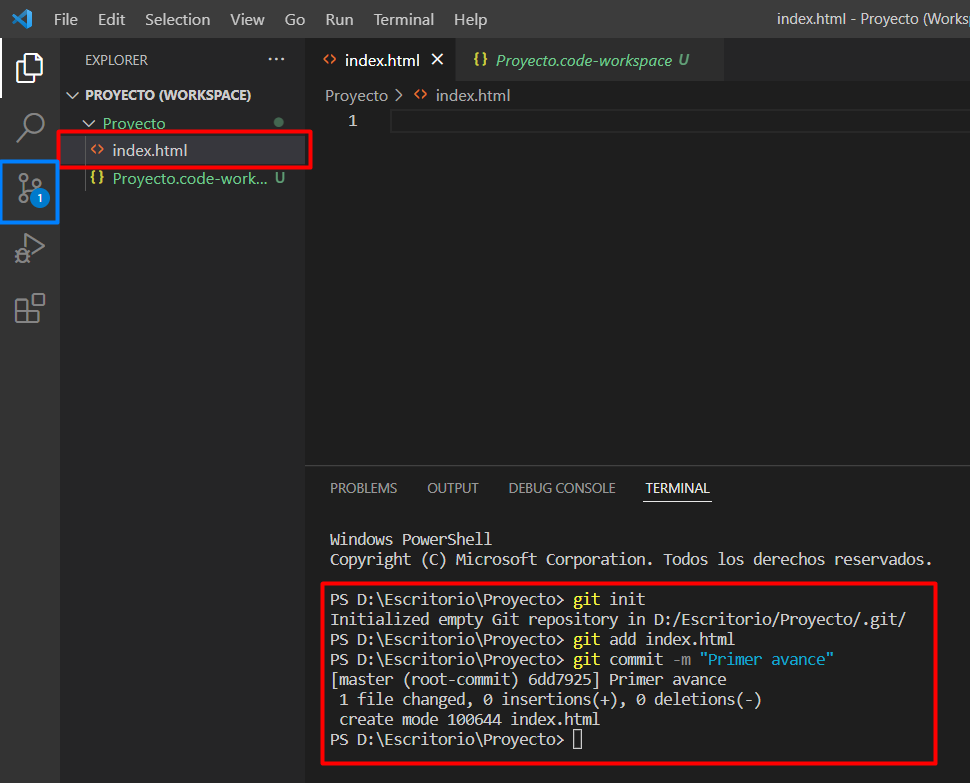
\includegraphics[width=12cm]{capturas/git add git commit.png}
\end{figure}

Ahora, realizaremos una modificación para ver el aspecto de VSC (\textit{Figura \ref{fig: 15}}):
\begin{figure}[H]
    \centering
    \caption{Seguimiento y commit de un archivo}
    \label{fig: 15}
    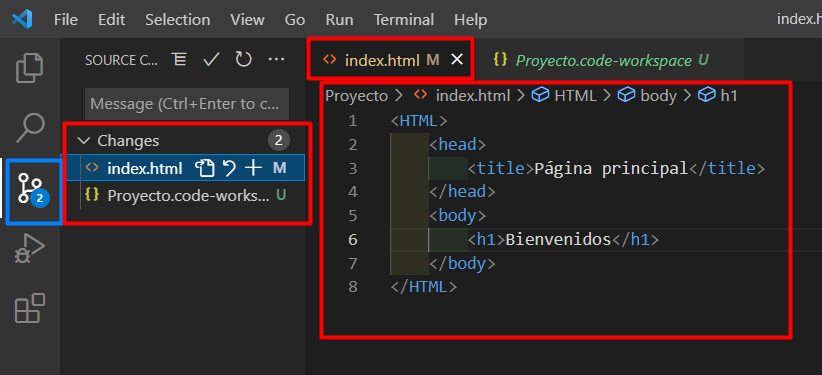
\includegraphics[width=12cm]{capturas/modificaciones.png}
\end{figure}

Otra vez, nuestra lista de tareas aumenta a 2 (recuadro azul), añadimos una estructura básica a \textit{index.html} y este tiene la letra M a su costado, podemos realizar un segundo commit. No olvide guardar todos los cambios en VSC y su Workspace antes de hacer un \textbf{git add} y \textbf{git commit}. Veamos la \textit{Figura \ref{fig: 16}} para ver el segundo commit.
\begin{figure}[H]
    \centering
    \caption{Segundo commit de nuestro proyecto}
    \label{fig: 16}
    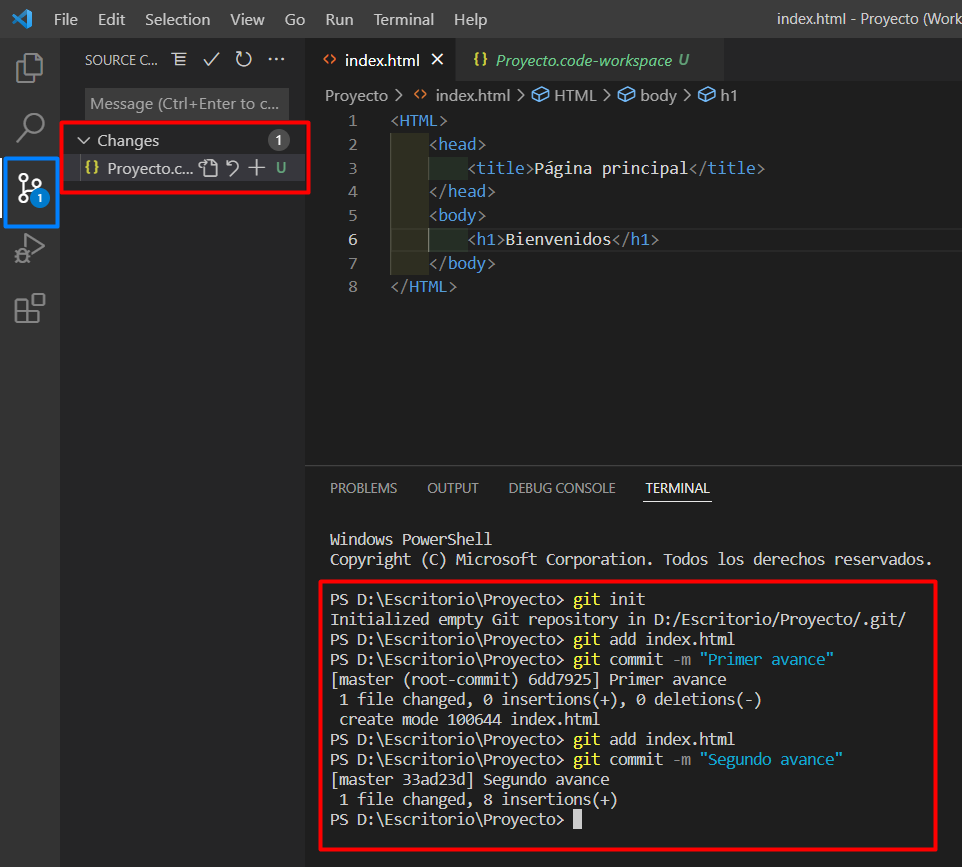
\includegraphics[width=12cm]{capturas/segundo commit.png}
\end{figure}

Las letras que aparecen significan:
\begin{itemize}
    \item \textbf{U}: unfollow, sin seguir, significa que los archivos no tienen seguimiento.
    \item \textbf{M}: modified, modificado, significa que a un archivo se le han hecho cambios, por lo que se le debe dar seguimiento nuevamente.
\end{itemize}



\section{VSC y sus herramientas visuales para trabajar con Git}
\hspace{0.55cm}Este editor cuenta con más herramientas que nos harán prescindir de la terminal.


\subsection{Creando ramas}

Por ejemplo, para \textbf{crear una rama} de Git en VSC podemos utilizar dos formas:
\begin{enumerate}
    \item \textbf{Con la barra de tareas inferior azul}: VSC posee una barra de tareas color azul en la parte inferior de su interfaz, donde suele mostrar los errores y alertas de un código, en que línea y columna estamos ubicados, entre otra información, en la zona izquierda de esta barra, encontramos un texto que nombra a la rama en donde estamos trabajando actualmente con nuestro proyecto en Git. Si damos clic sobre este texto, nos abre una barra de acciones en la parte superior central de VSC dándonos algunas opciones, como la de \textbf{Crear rama} y ver las ramas existentes, como se ve en la \textit{Figura \ref{fig: 17}}:
    \begin{figure}[H]
        \centering
        \caption{Creando una rama con VSC y su barra de tareas}
        \label{fig: 17}
        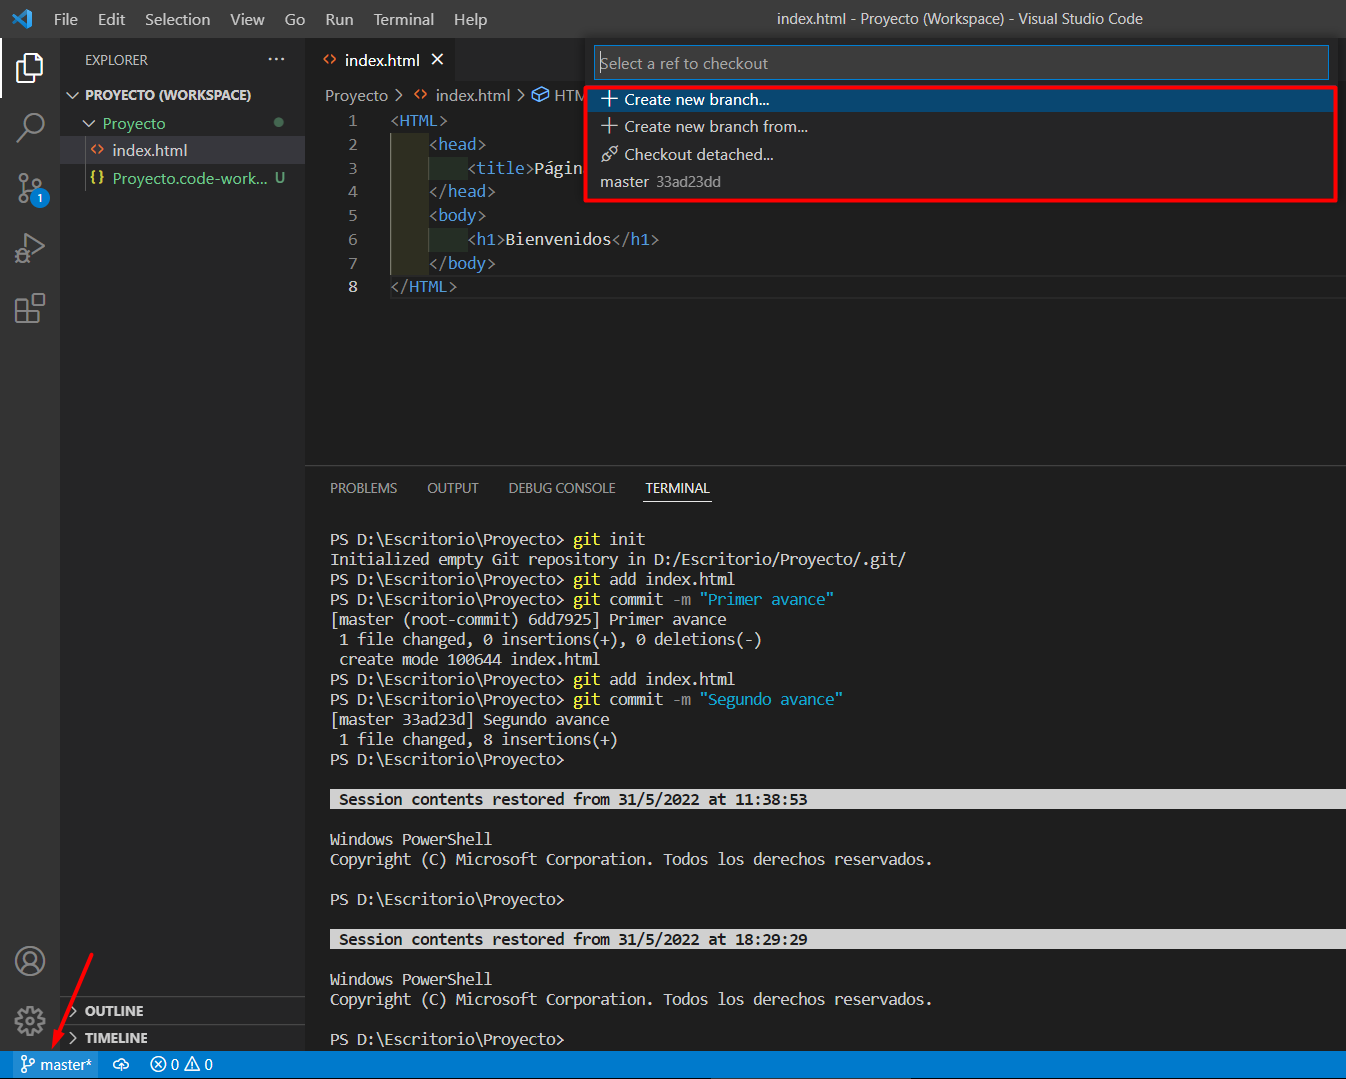
\includegraphics[width=\textwidth]{capturas/creando_b1.png}
    \end{figure}
    
    Al dar clic en \textbf{Create new branch...} nos pedirá el nombre de esta, una vez escrito, damos ENTER para continuar y la rama se ha creado, VSC nos sitúa en la rama recién creada para comenzar a trabajar en ella directamente. Si volvemos a dar clic sobre el nombre de la rama en la barra de tareas, él menú desplegado, además de darnos la posibilidad de crear otra rama, nos muestra las dos existentes hasta el momento, como se ve en la \textit{Figura \ref{fig: 18}}:
    \begin{figure}[H]
        \centering
        \caption{Cambiando entre ramas con VSC}
        \label{fig: 18}
        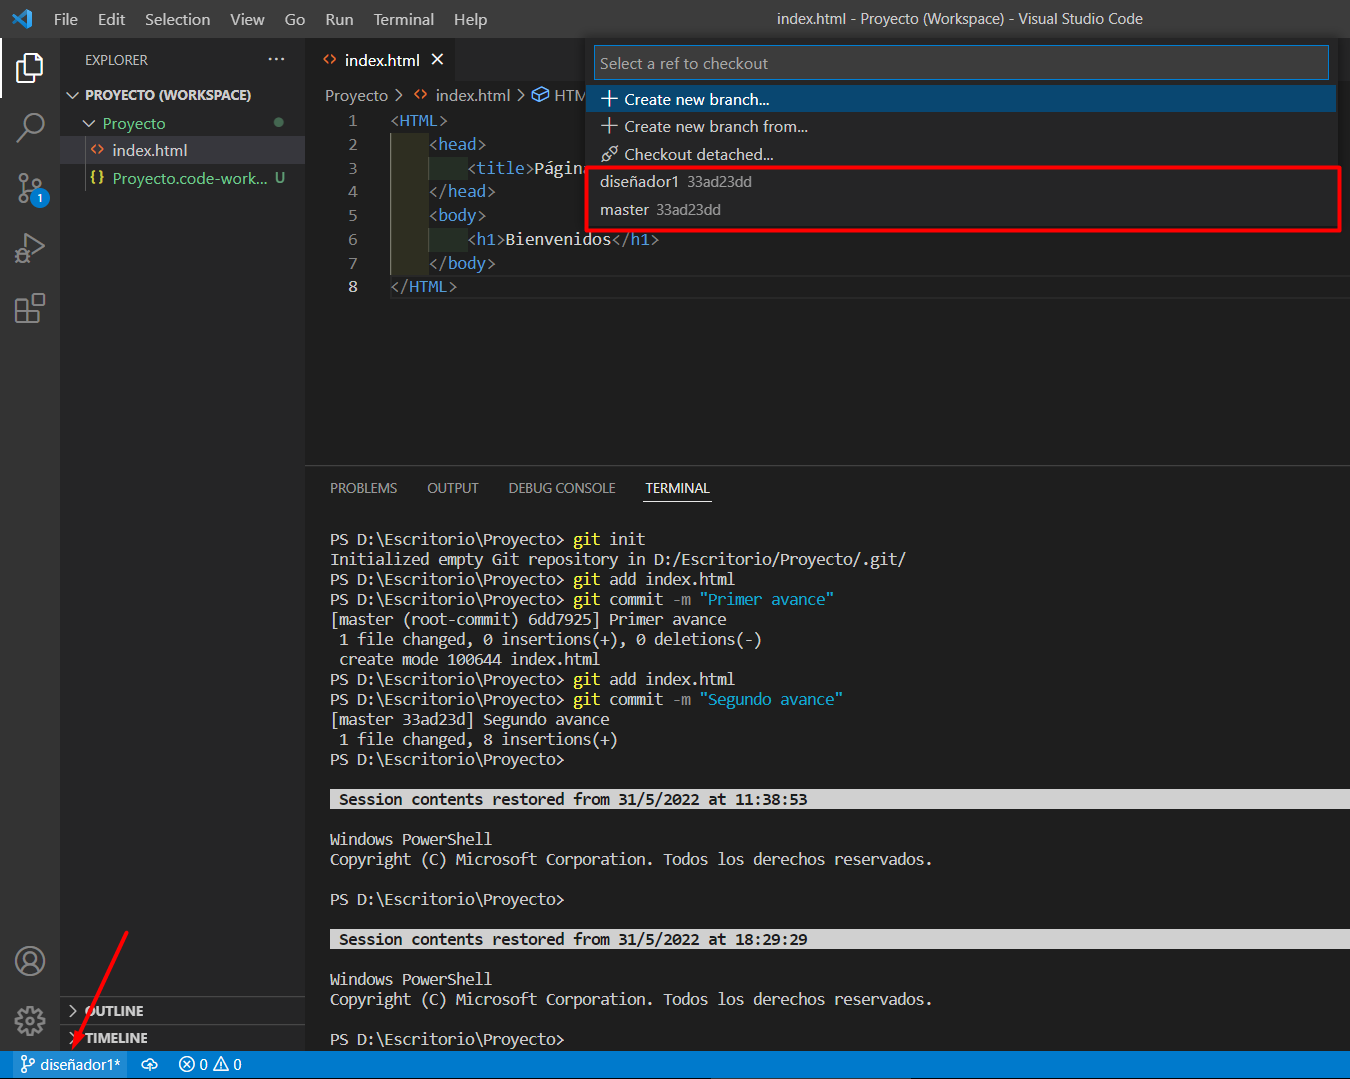
\includegraphics[width=\textwidth]{capturas/abriendo_b1.png}
    \end{figure}
    
    \item \textbf{Con el menú de tareas lateral y sus tres puntos}: esta opción es un poco más completa, y nos sitúa en un espacio donde aparecen muchas más opciones para trabajar con Git. Nos vamos a la opción de tareas de Git, en este punto, tenemos una tarea pendiente, que es darle seguimiento al archivo de Workspace de nuestro proyecto, pero lo dejaremos como está, vemos que encima de \textbf{Changes} hay una caja de texto para escribir algo, encima de esta, hay un botón con la forma de tres puntos, si damos clic a dicho botón, se nos despliegan múltiples características Git que podemos usar, entre ellas, está la opción \textbf{Branch}, si la seleccionamos, podemos encontrar la opción de \textbf{Create branch...}, además de las opciones para unir ramas, renombrar alguna, borrar, entre más, como vemos en la \textit{Figura \ref{fig: 19}}:
    \begin{figure}[H]
        \centering
        \caption{Creando una rama con VSC y la opción de tareas}
        \label{fig: 19}
        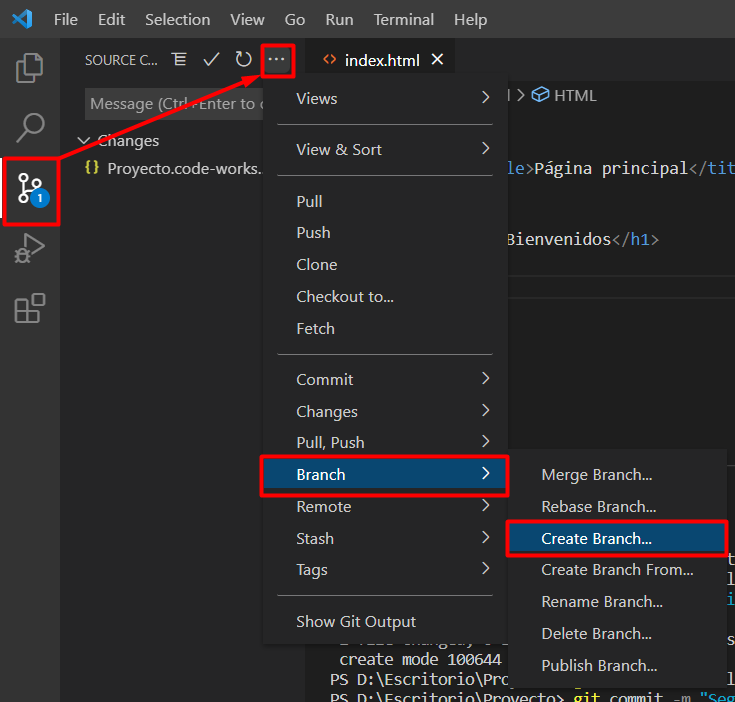
\includegraphics[width=\textwidth]{capturas/creando_b2.png}
    \end{figure}
\end{enumerate}


\subsection{Agregando archivos al área de ensayo}

Nos quedaremos en la rama diseñador1. Este punto es bastante simple, si realizo alguna modificación en \textit{index.html}, sabemos que este archivo aparecerá en el menú de tareas de Git, si situamos el puntero del mouse encima del archivo con letra M, veremos que aparecen varias opciones, entre ellas, un icono de Más (+), el cual realiza la tarea de agregar el archivo al área de ensayo, lo único que debemos hacer es darle clic, y nuestro archivo tendrá seguimiento (\textit{Figura \ref{fig: 20}}).
\begin{figure}[H]
    \centering
    \caption{Agregando archivos al área de ensayo con VSC}
    \label{fig: 20}
    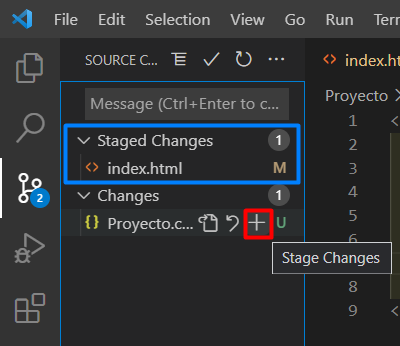
\includegraphics[width=10cm]{capturas/seguimiento_archivos.png}
\end{figure}

El archivo \textit{index.html} ya tiene seguimiento, lo vemos encerrado en el recuadro azul, mientras que el archivo de Workspace no lo tiene, por eso aparece el botón + entre sus opciones.


\subsection{Realizando commits}

Aquí se nos presenta una opción bastante útil en caso de tener varios archivos. Como dijimos anteriormente, hay una caja de texto en el menú de tareas en la cual podemos ingresar un texto, este texto es el mensaje que tendrá un commit, al escribirlo y dando CTRL + ENTER, se llevará a cabo un commit, pero el alcance que este tendrá solo aplicará a los archivos que tienen seguimiento (\textit{Figura \ref{fig: 21}}).
\begin{figure}[H]
    \centering
    \caption{Commit con caja de texto}
    \label{fig: 21}
    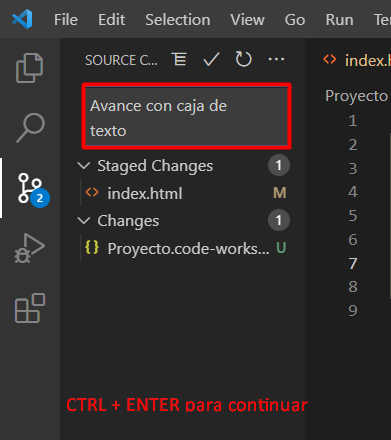
\includegraphics[width=10cm]{capturas/commits1.png}
\end{figure}

En cambio, si repetimos la acción de escribir el mensaje, teniendo archivos con y sin seguimiento (letra M y U) y presionamos el botón con una palomita, VSC nos lanzará una alerta que dice que si queremos realizar el commit usando todos los archivos (con y sin seguimiento) siempre, nunca o solo en esta ocasión, nosotros diremos que solo en esta ocasión (\textit{Figura \ref{fig: 22}}).
\begin{figure}[H]
    \centering
    \caption{Commit con botón de palomita}
    \label{fig: 22}
    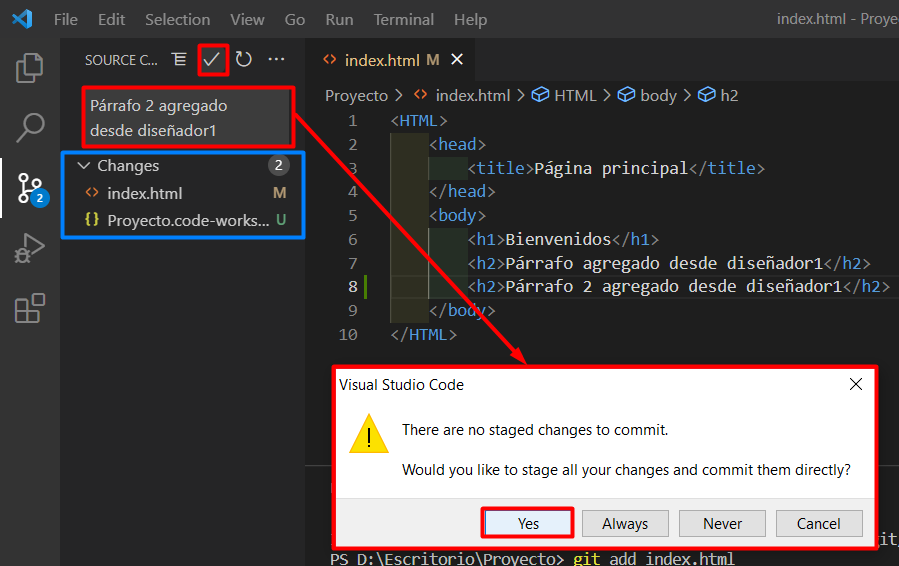
\includegraphics[width=13cm]{capturas/commits2.png}
\end{figure}

Y si recordamos cómo crear ramas con VSC, sabremos que si damos clic al botón de los tres puntos, ahí también aparece la opción de commits.


\subsection{Unir ramas y conflictos de concurrencia}

Una vez terminado el trabajo en dos ramas distintas, damos clic al botón de los tres puntos en el menú de tareas, dentro de la opción \textbf{Branch}, encontramos la opción \textbf{Merge branch...}, VSC toma la rama donde estamos trabajando como rama inicial, y nos despliega una lista de las demás ramas para unirlas, como vemos en la \textit{Figura \ref{fig: 23}} y \textit{Figura \ref{fig: 24}}:
\begin{figure}[H]
    \centering
    \caption{Uniendo varias ramas}
    \label{fig: 23}
    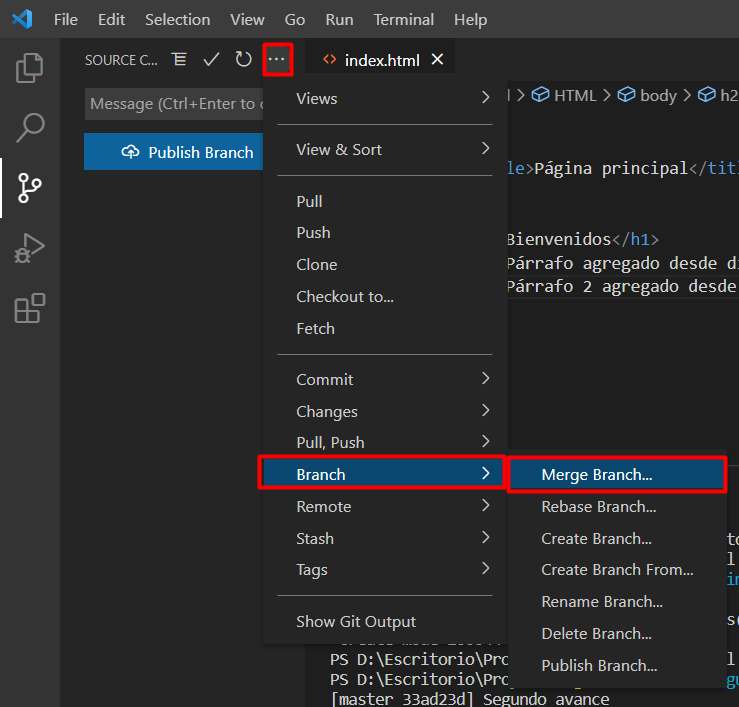
\includegraphics[width=10cm]{capturas/merge1.png}
\end{figure}
\begin{figure}[H]
    \centering
    \caption{Selección de ramas para unir}
    \label{fig: 24}
    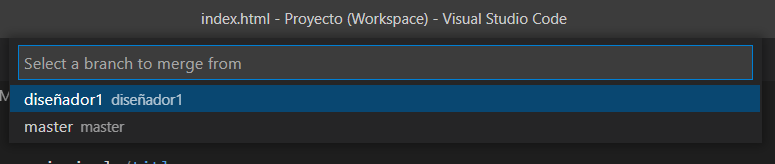
\includegraphics[width=\textwidth]{capturas/merge2.png}
\end{figure}

Esto en caso de que no hubiera ningún conflicto de concurrencia, pongamos la siguiente situación: en \textbf{master}, agregamos más texto al \textbf{Header 1} y hacemos un commit, en \textbf{diseñador1} volvemos a hacer cambios en el \textit{Header 1} y volvemos a realizar un commit, finalmente, realizamos el proceso de unión de ramas, sin embargo, hicimos un problema de concurrencia a propósito para ver como lo trata VSC en la \textit{Figura \ref{fig: 25}}:
\begin{figure}[H]
    \centering
    \caption{Uniendo varias ramas con un problema de concurrencia}
    \label{fig: 25}
    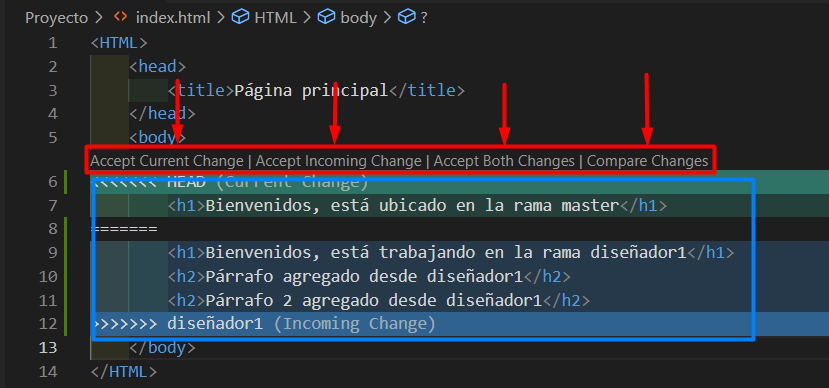
\includegraphics[width=13cm]{capturas/merge3.png}
\end{figure}

Vemos que VSC nos lanza una advertencia de que hay un problema de concurrencia, en \textbf{master} y en \textbf{diseñador1} se han realizado cambios en la misma línea de código, por lo que se nos ofrecen las siguientes opciones: aceptar el cambio de la rama actual, aceptar el cambio de la rama con la que se desea mezclar, aceptar ambos cambios y comparar ambos cambios, dependiendo de nuestras necesidades, aceptamos una u otra, nosotros aceptaremos los dos cambios.

Una vez escogida la opción, VSC da seguimiento al archivo donde ocurrió el problema, escribe un texto en la caja de mensaje para realizar un commit, se puede dejar o se puede cambiar, y podemos realizar el commit con el archivo ya mezclado sin problemas (\textit{Figura \ref{fig: 26}})
\begin{figure}[H]
    \centering
    \caption{Uniendo varias ramas después de un problema de concurrencia}
    \label{fig: 26}
    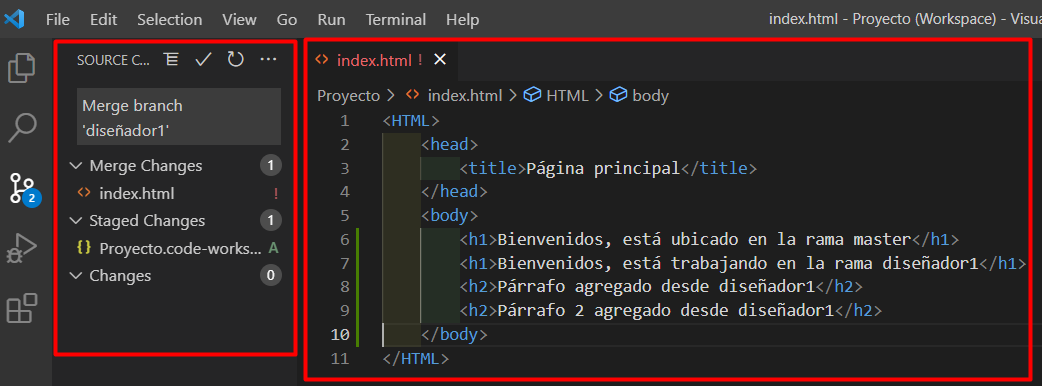
\includegraphics[width=13cm]{capturas/merge4.png}
\end{figure}

\textit{Nota}: en caso de que se presente algún error para realizar el commit en este punto, puede poner el puntero del mouse encima del archivo que tuvo los problemas de concurrencia y dar clic al botón de +, para darle seguimiento.


\subsection{Sincronizando y subiendo proyecto de VSC a GitHub}

Podemos subir nuestro proyecto a GitHub de dos formas, desde el \textbf{panel de tareas de Git} y desde la \textbf{barra de tareas de VSC}, en nuestra situación, no hemos ingresado ninguna cuenta de GitHub ni enlace de repositorio, por lo que, para ambas opciones, VSC nos pedirá que ingresemos la información mencionada. Los recuadros azules en la \textit{Figura \ref{fig: 27}} muestran la ubicación de las dos opciones para subir proyectos desde VSC:
\begin{figure}[H]
    \centering
    \caption{Subir proyectos a GitHub desde VSC}
    \label{fig: 27}
    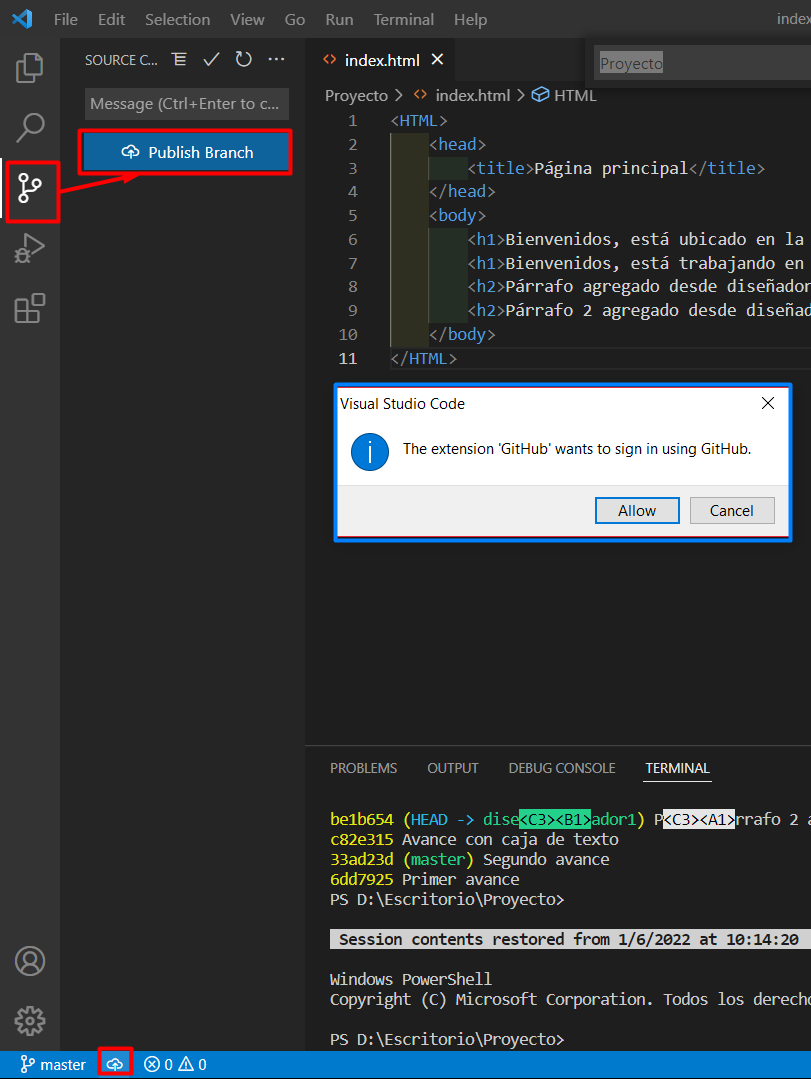
\includegraphics[height=13cm]{capturas/subir_proyecto1.png}
\end{figure}

En caso de que, en tu navegador estés loggeado en GitHub, VSC solamente te pedirá que des clic a un botón para dar autorización a GitHub de poder trabajar en VSC y que ingreses tu contraseña, en caso contrario, pedirá que ingreses tu correo, contraseña, y des autorización.

Una vez iniciada sesión en GitHub con VSC, este último te preguntará a qué tipo de repositorio subir tu proyecto local: si a un repositorio público o privado, escoge alguna opción, posterior a ello, comenzará el proceso para subir el proyecto local a GitHub, debes tener en cuenta de que, cuando se suba, VSC creará un repositorio en GitHub con el mismo nombre del proyecto local y ahí lo publicará.

Si realizamos alguna modificación en el archivo \textit{index.html} y realizamos un commit nuevo, para subir este cambio a GitHub, presionamos alguna de las dos opciones mostradas en la \textit{Figura \ref{fig: 28}} para subir nuestros cambios, a esta acción se le conoce como \textbf{push}:
\begin{figure}[H]
    \centering
    \caption{Subir cambios del proyectos a GitHub desde VSC}
    \label{fig: 28}
    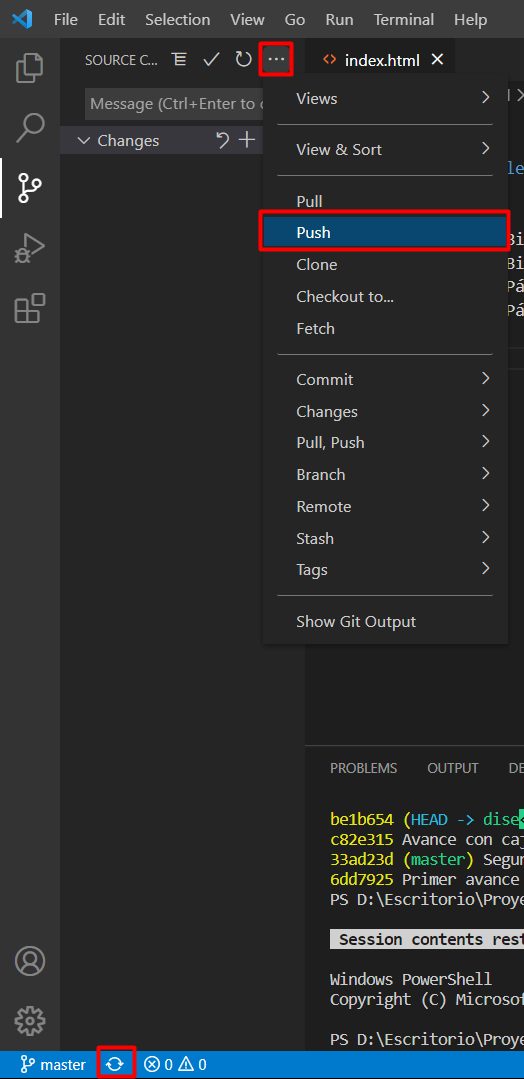
\includegraphics[height=13cm]{capturas/subir_proyecto2.png}
\end{figure}

Si previamente ya teníamos un repositorio creada en GitHub donde deseamos que se suba nuestro proyecto local, podemos acudir a la \textbf{Paleta de comandos} para poder obtener acceso a los comandos que ya conocemos de Git de una forma más visual y fácil de comprender. Abrimos la \textit{Paleta de comandos} yéndonos al opción \textbf{View} en la barra superior de VSC, la primer opción desplegada es la que requerimos. Una vez aparece la barra, escribimos la palabra "git" y, en ese momento, se nos abren todos los comandos de Git permitidos en VSC, estando en ese menú, podemos buscar el comando \textbf{Git: Add Remote...}, ahí escribiremos la dirección del repositorio que ya tenemos creado, como vemos en la \textit{Figura \ref{fig: 29}} y \textit{\ref{fig: 30}}.
\begin{figure}[H]
    \centering
    \caption{Subir proyecto a GitHub con la Paleta de comandos}
    \label{fig: 29}
    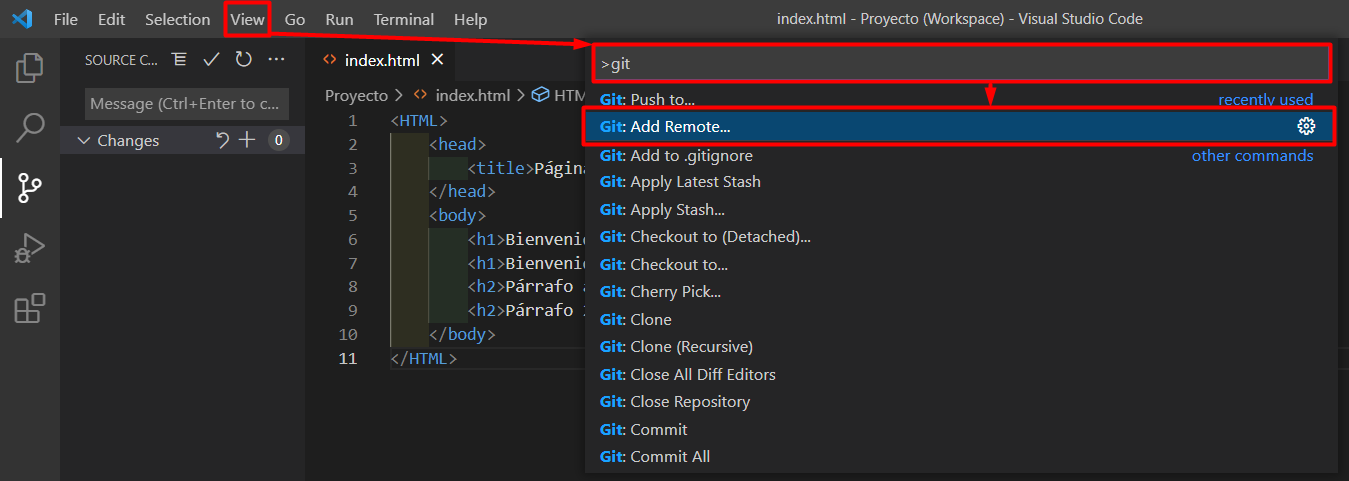
\includegraphics[width=13cm]{capturas/subir_proyecto3.png}
\end{figure}
\begin{figure}[H]
    \centering
    \caption{Agregar dirección de repositorio GitHub a VSC}
    \label{fig: 30}
    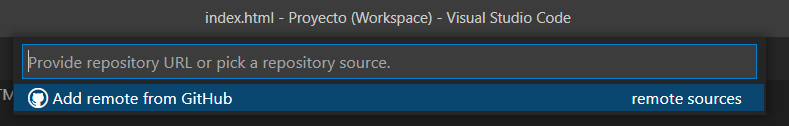
\includegraphics[width=13cm]{capturas/subir_proyecto4.png}
\end{figure}

Una vez agregado el repositorio a VSC, volvemos a abrir la Paleta de comandos, escribimos "git" y buscamos el comando \textbf{Git: Push To...} (\textit{Figura \ref{fig: 31}}) y lo seleccionamos; en este punto, tenemos la dirección del repositorio que se creó automáticamente cuando agregamos nuestra cuenta de GitHub a VSC y la dirección del repositorio que acabamos de añadir, seleccionamos la dirección más reciente y el proyecto se habrá subido.
\begin{figure}[H]
    \centering
    \caption{Subir proyecto a GitHub en un repositorio existente}
    \label{fig: 31}
    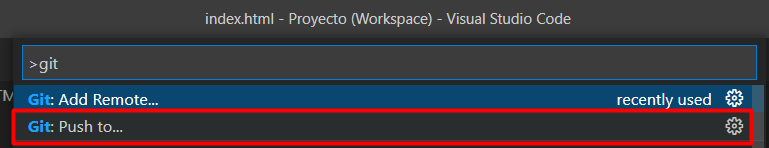
\includegraphics[width=13cm]{capturas/subir_proyecto5.png}
\end{figure}

Como vemos, para subir un proyecto local a GitHub primero debemos estar loggeados en VSC con nuestra cuenta de GitHub, con esa información, VSC detecta crea automáticamente un repositorio online con el mismo nombre que el proyecto local, subiendo ahí nuestro trabajo, sin embargo, si buscamos que se suba a otro repositorio, debemos agregar la dirección de este a VSC con el comando \textbf{Add Remote...} y, posterior a ello, utilizar el comando \textbf{Push To...}.

Sabemos que se pueden editar archivos en GitHub, si en nuestro archivo \textit{index.html} le agregamos un párrafo desde GitHub y queremos que aparezca en VSC, simplemente debemos darle clic al icono de \textbf{sincronización} en la \textbf{barra de tareas} (\textit{Figura \ref{fig: 32}}). Para que aparezca el cambio de VSC a GitHub, realizamos el commit con nuestros cambios y realizamos un push a el repositorio que deseemos.
\begin{figure}[H]
    \centering
    \caption{Subir proyecto a GitHub en un repositorio existente}
    \label{fig: 32}
    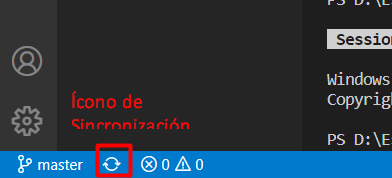
\includegraphics[width=10cm]{capturas/sincronizacion.png}
\end{figure}

Si queremos ahorrarnos el paso de la creación de un repositorio automático para, posterior, agregar la dirección del repositorio que realmente queremos trabajar, siga los pasos de la siguiente sección.


\subsection{Clonación de proyectos}

Con la dirección del repositorio que queremos pasar de GitHub a VSC, nos vamos al editor de texto, en el \textbf{Panel de tareas de Git} o \textbf{Paleta de comandos} buscamos la operación \textbf{Clone}, como vemos en la \textit{Figura \ref{fig: 33}}.
\begin{figure}[H]
    \centering
    \caption{Opciones para clonar un repositorio online a local}
    \label{fig: 33}
    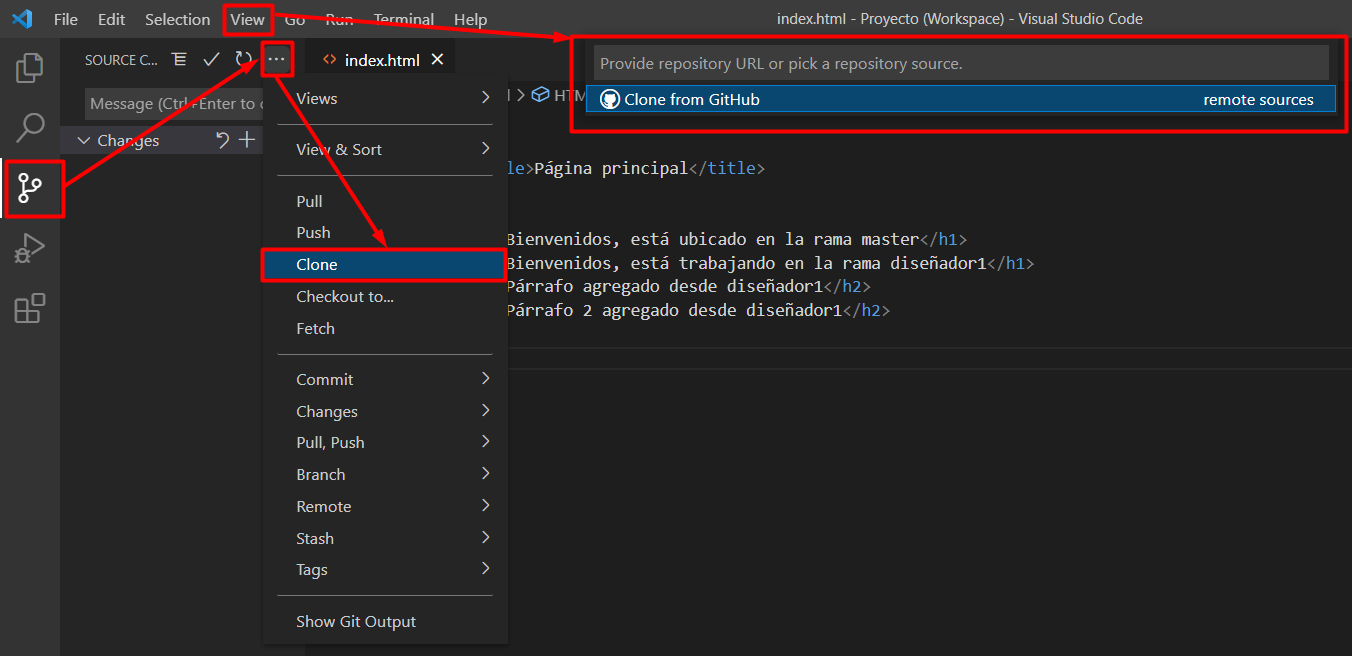
\includegraphics[width=13cm]{capturas/clone.png}
\end{figure}

En ambas situaciones, debemos escribir en la caja de texto la dirección \textbf{.git} del repositorio online que buscamos clonar, posterior a ello, VSC nos mostrará un Explorador de archivos para seleccionar una carpeta donde guardar todos los archivos del repositorio online y, finalmente, comenzará el proceso de clonación, después de esperar un poco, tendremos el repositorio online en nuestra máquina.



\section{Trabajando en GitHub}

Nos alejaremos un poco de VSC, en esta sección, simplemente vamos a destacar algunas herramientas o funciones que nos ofrece GitHub en su plataforma en línea. Ingresamos a \href{https://github.com/}{Github} e iniciamos sesión en nuestra cuenta, accedemos a cualquier repositorio en línea con el que contemos, en esta ocasión, mostraremos como prueba el repositorio que hemos utilizado previamente en estos apuntes (pruebaGIT), la \textit{Figura \ref{fig: 34}} muestra algunos de sus funciones y componentes:
\begin{figure}[H]
    \centering
    \caption{Componentes y funciones de GitHub}
    \label{fig: 34}
    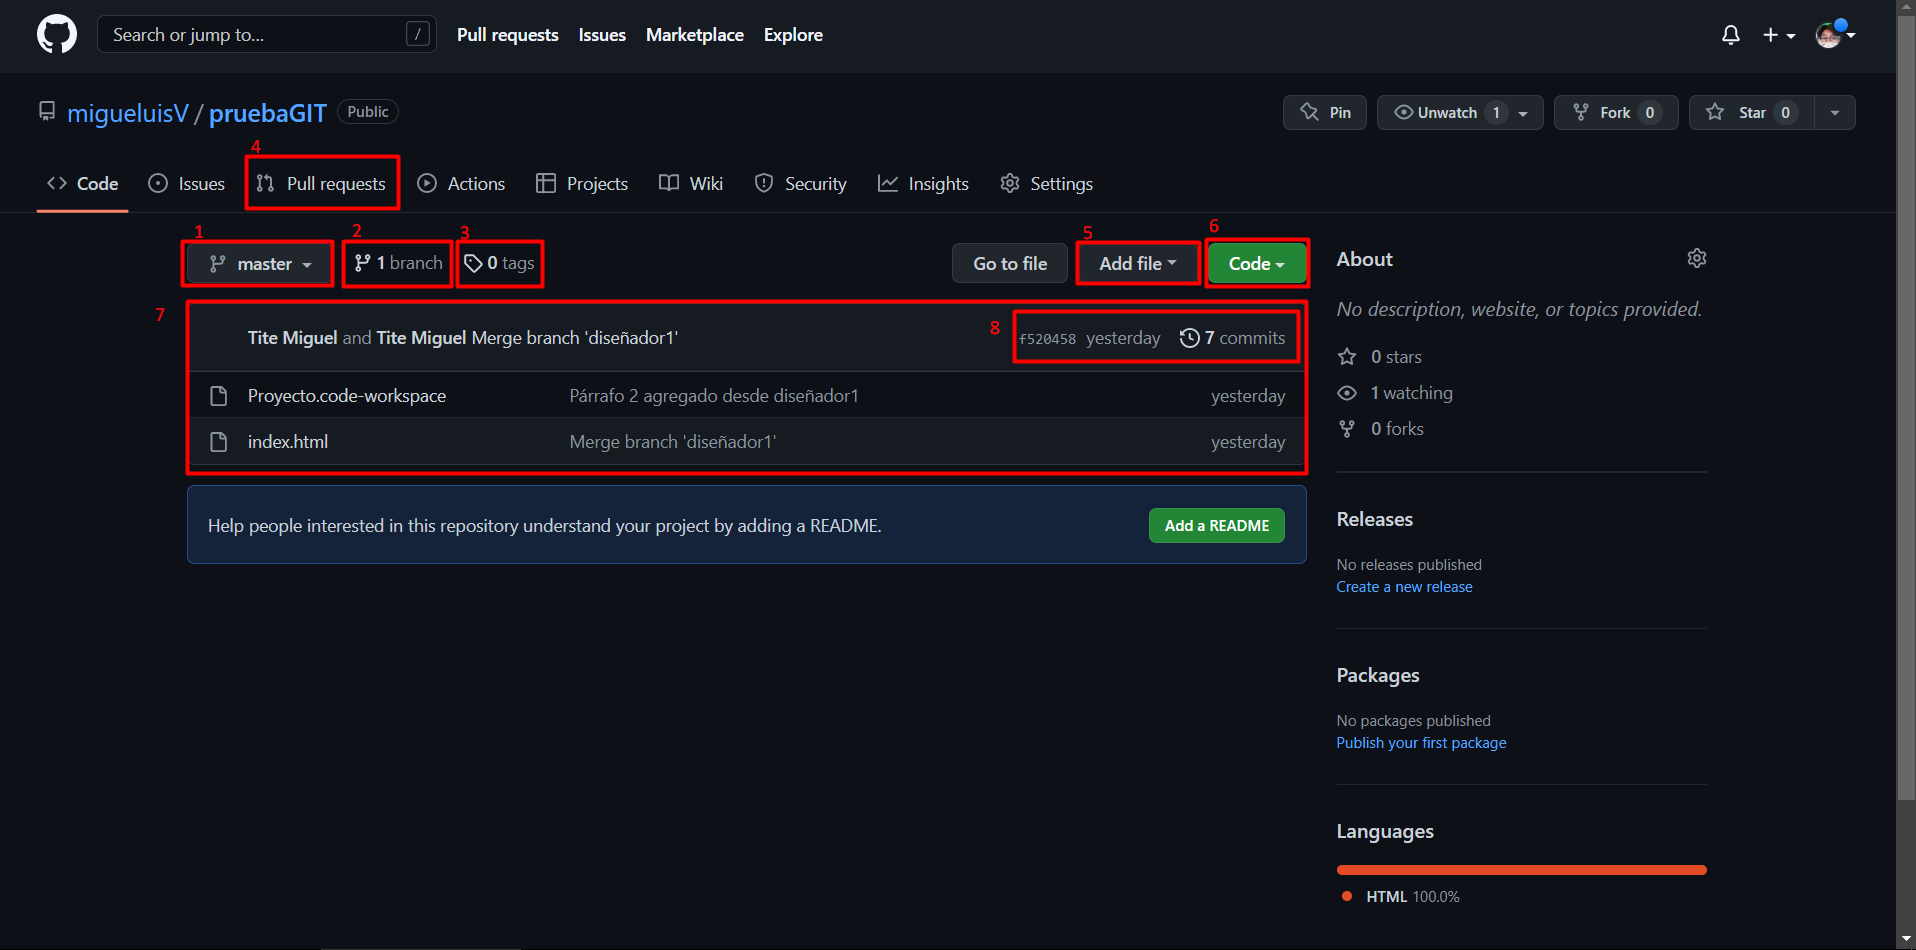
\includegraphics[width=\textwidth]{capturas/github.png}
\end{figure}

Donde:
\begin{enumerate}
    \item muestra la rama donde actualmente estamos trabajando, muestra todos los archivos de la rama.
    \item muestra la cantidad de \textbf{ramas} existentes en el repositorio.
    \item muestra la cantidad de \textbf{etiquetas} existentes en el repositorio.
    \item muestra las \textbf{solicitudes de mezcla de ramas} pendientes por revisar y aprobar.
    \item opción para \textbf{agregar un archivo} de nuestra computadora o crearlo en GitHub.
    \item muestra la dirección \textbf{.git} de nuestro repositorio.
    \item muestra todos los archivos de una rama del repositorio.
    \item muestra la \textbf{cantidad de commits} que posee la rama.
\end{enumerate}



\section{Fork}

Si recordamos el concepto de \textit{ramas}, sabemos que es la copia de los archivos de nuestro proyecto para que más de una persona pueda trabajar en nuestro repositorio, al final, se mezclan ambas ramas para que se unifique el proyecto, entonces, el concepto de \textbf{fork} va más allá de una rama, sigue la misma lógica que las ramas, pero a escala de repositorios. Un \textit{fork} es la copia del repositorio de un usuario en nuestra cuenta o cuenta de algún usuario que se haya visto interesado en el repositorio que busca copiar, el usuario original puede realizar commits y modificaciones en su trabajo original, mientras que el usuario que tiene una copia del repositorio puede clonarlo y hacer lo mismo, el usuario con el repositorio fork puede realizar una solicitud de merge al usuario propietario y este puede aceptarla, comentarla, revisarla, compararla o declinarla. La \textit{Figura \ref{fig: 35}} muestra como se ven un repositorio propietario y uno fork:
\begin{figure}[H]
    \centering
    \caption{Ejemplificación de un repositorio propietario y uno fork}
    \label{fig: 35}
    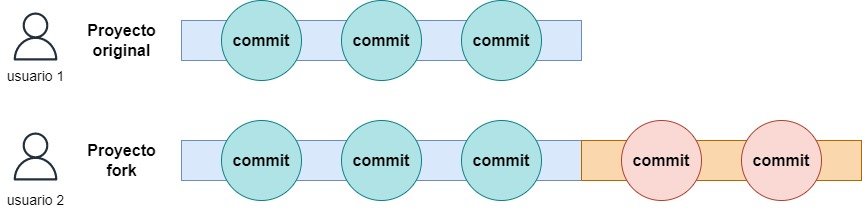
\includegraphics[width=13cm]{capturas/fork1.jpg}
\end{figure}

Si vamos a un repositorio nuestro en GitHub en la esquina superior derecha, aparece un botón con el texto \textbf{Fork} (\textit{Figura \ref{fig: 36}}) y \textit{\ref{fig: 37}}:
\begin{figure}[H]
    \centering
    \caption{Ubicación del botón Fork en GitHub}
    \label{fig: 36}
    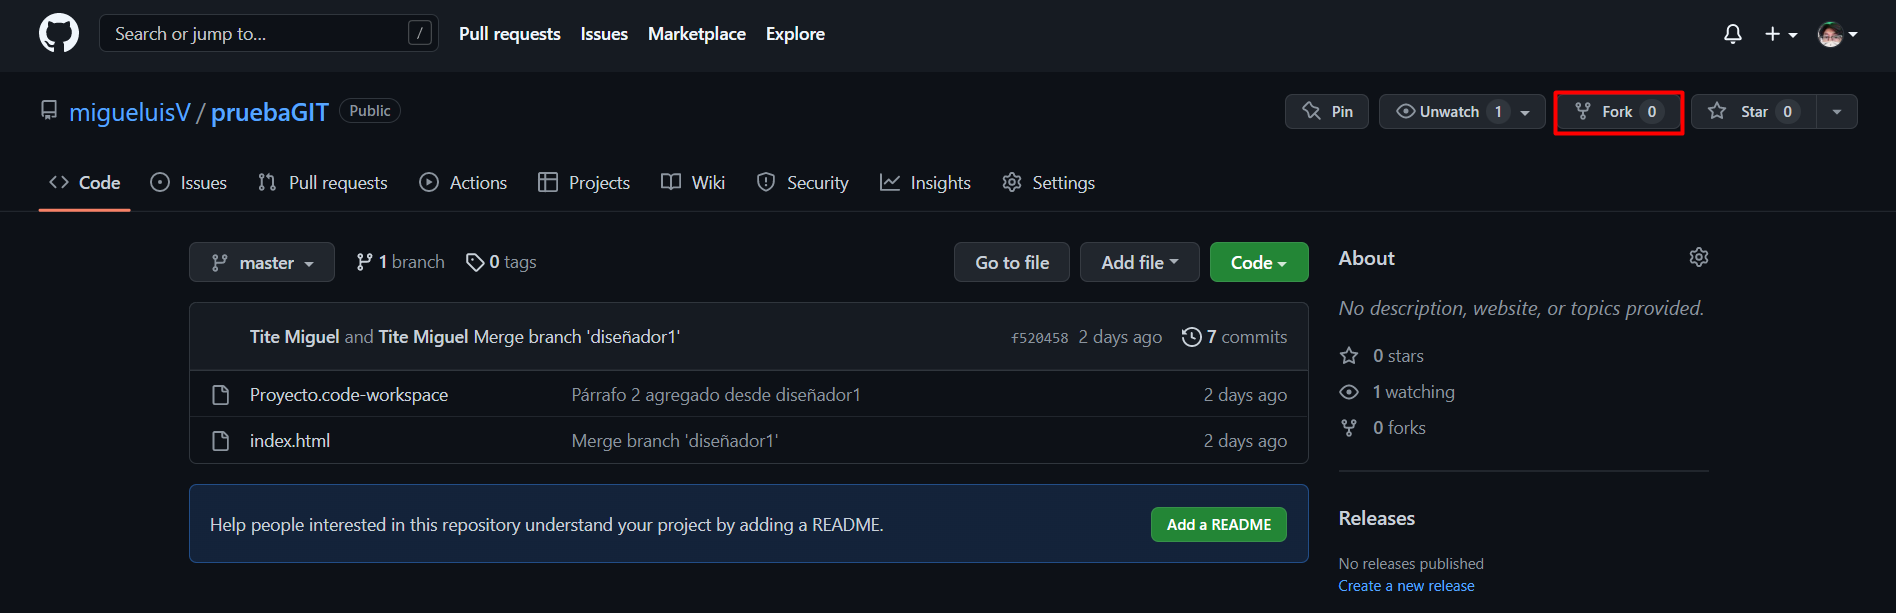
\includegraphics[width=13cm]{capturas/fork2.png}
\end{figure}
\begin{figure}[H]
    \centering
    \caption{Menú de Fork}
    \label{fig: 37}
    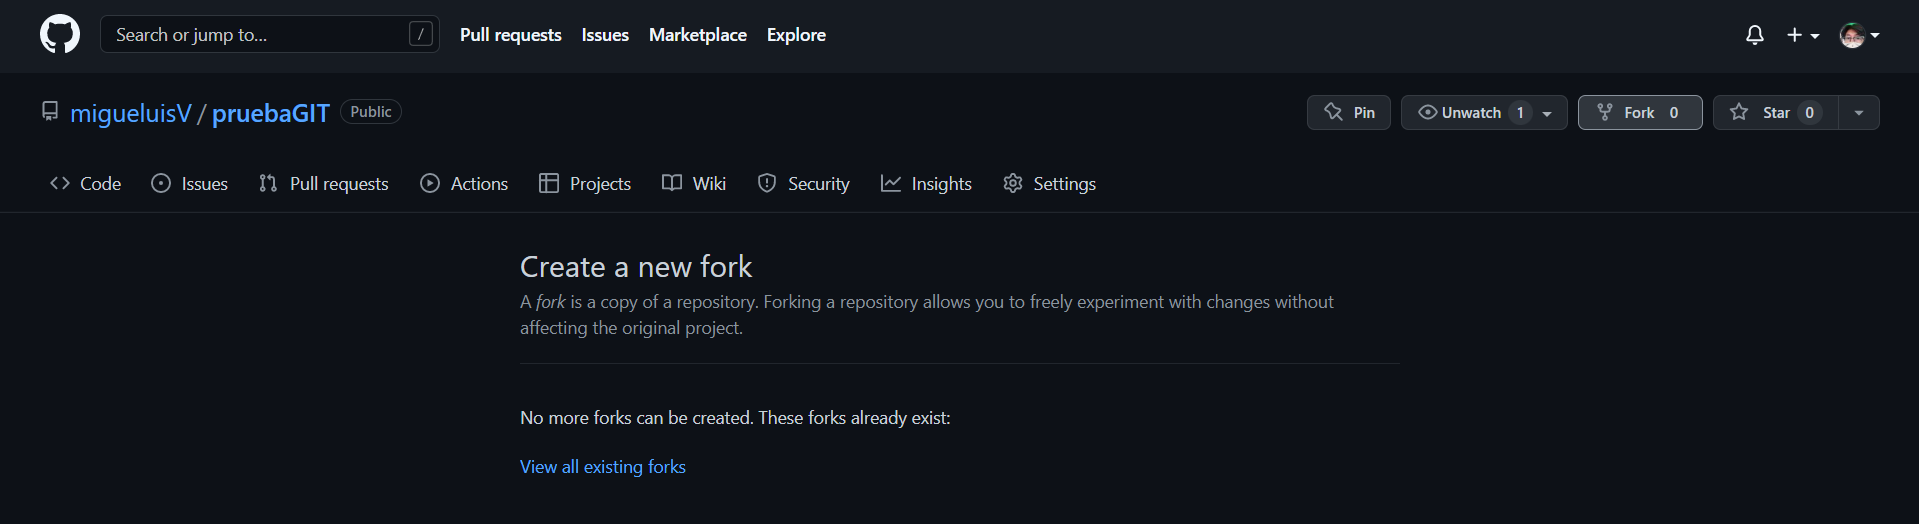
\includegraphics[width=13cm]{capturas/fork3.png}
\end{figure}

Como es nuestro propio proyecto, no podemos crear un fork, sin embargo, si estuviésemos en una cuenta distinta, buscamos nuestro usuario, y buscamos el repositorio en que estamos interesados, el mismo botón \textbf{Fork} está ubicado donde mismo, le damos clic y debe aparecer un texto para realizar un \textit{fork} a los repositorios de la cuenta externa.

Algo que se debe tomar en consideración es que previamente, a lo largo de este documento, ingresamos las credenciales de GitHub de una cuenta (cuenta A), ya sea en la consola o en VSC para poder hacer \textbf{push} y \textbf{commits} de nuestros proyectos a GitHub, entonces, la información de la cuenta A fue almacenada en el sistema donde estemos trabajando, en nuestro caso, Windows, así que, si realizamos un fork de un repositorio A de la cuenta A a una cuenta B (repositorio B) en GitHub, debemos de salir de la cuenta A para ingresar como la cuenta B en nuestra computadora para trabajar el repositorio B, para hacer esto, debemos \textbf{eliminar las credenciales} del sistema, revise el siguiente subtítulo.


\subsection{Eliminando credenciales de GitHub de Windows}

Damos clic en el botón de \textbf{Windows}, abrimos la \textbf{Configuración}, escribimos en la barra de búsqueda "credenciales" y abrimos el programa \textbf{Administrador de credenciales}, abierto el programa, damos clic a la opción \textbf{Credenciales de Windows} y buscamos aquella que se llame \textbf{git:https://github.com}, simplemente damos clic sobre esta credencial, se abre un pequeño menú y damos clic a la opción \textbf{Quitar}, como se ve en la \textit{Figura \ref{fig: 38}}.
\begin{figure}[H]
    \centering
    \caption{Eliminando credencial de GitHub en Windows}
    \label{fig: 38}
    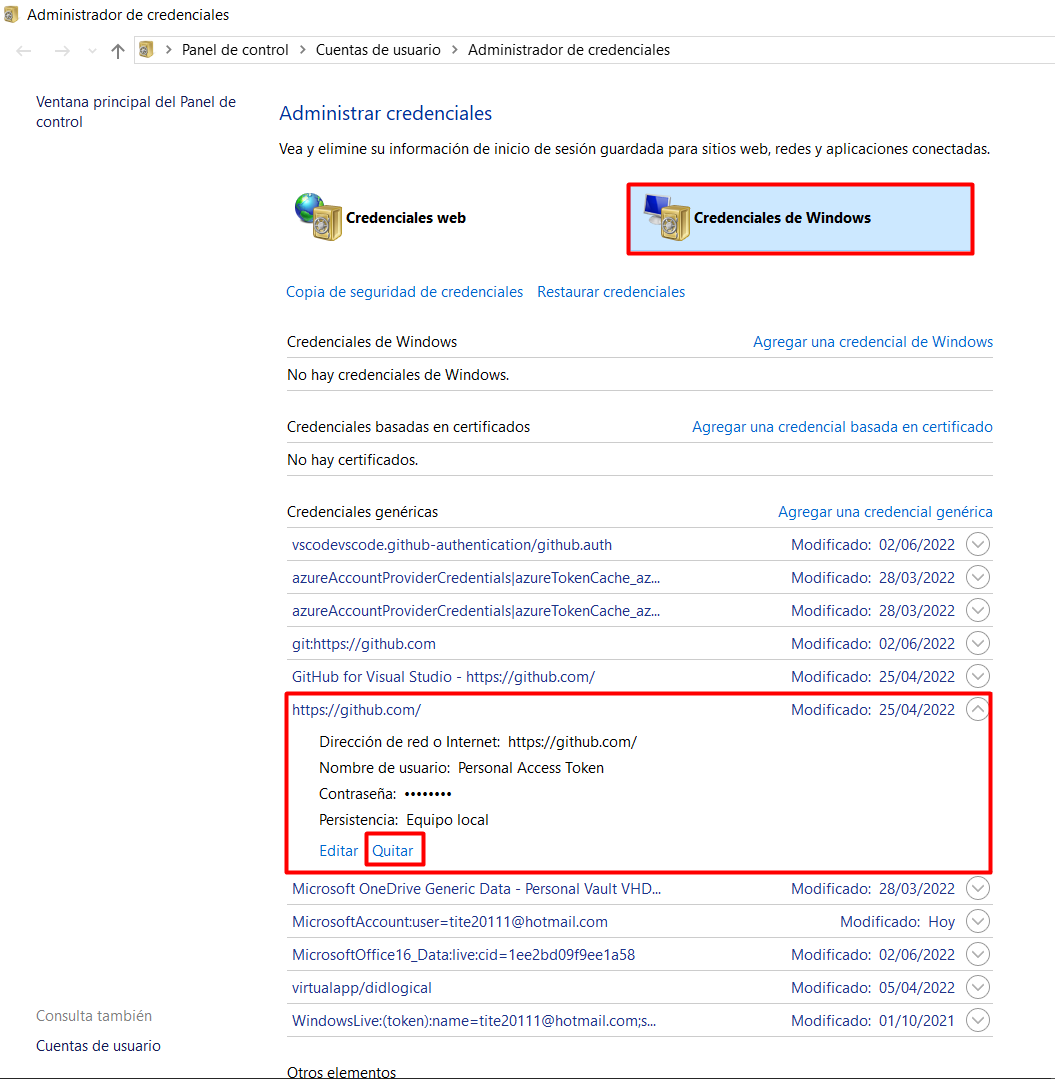
\includegraphics[height=13cm]{capturas/credencial.png}
\end{figure}

Con esto, podemos volver a iniciar sesión en Git o VSC con una cuenta B o diferente a la cuenta A y, como resultado, poder trabajar los repositorios de la cuenta B o repositorios \textit{fork}.
